\chapter{Jet Results and Discussion} \label{ch:analysis}

Beginning in March of 2012, the LHC began seven months of pp collisions at $\sqrt{s} = \,$ 8 TeV.  The jet cross sections and ratios of the cross sections for jets of different radii offers a unique perspective on the pQCD effects of hadronization at this new energy frontier.  Due to the expectation that no QGP is formed in a pp collision these measurements serve as a baseline for separating phenomena associated with the QGP in heavy-ion collisions.  In order to measure the jet cross section the following formula is used,

\begin{equation}
	\frac{d^{2} \sigma^{jet}}{d\eta \, dp_{T}} = \frac{A_{trigger}}{\epsilon_{trigger}(p_{T})} \times C_{MC} \times \frac{1}{A(p_{T}) } \times \frac{1}{\mathscr{L}_{int}} \times \frac{dN^{2}_{jet}}{dp_{T} \, d\eta}
\label{eq:xsecdef}
\end{equation}

\noindent
where,

\begin{itemize}
  \item $A_{trigger}$ is the acceptance for EMCal triggered events and $\epsilon_{trigger}(p_{T})$ is the EMCal trigger efficiency.  These factors correct for imperfections in the electronics of the EMCal and the overall factors are equal to one in minimum bias events.
  \item $C_{MC}$ is a correction factor due to detector effects and it allows for comparisons between the ALICE experiment to other experiments or theoretical calculations.  Unfolding is used to determine this factor.
  \item $\mathscr{L}_{int}$ is the integrated luminosity during the period when the data was recorded.
  \item $A(p_{T})$ is the geometrical detector acceptance.
  \item $\frac{dN^{2}_{jet}}{dp_{T} \, d\eta}$ is the inclusive jet momentum spectra.
  
\end{itemize}

\noindent
Furthermore, it is useful to define the ratio of cross sections,

\begin{equation}
\mathscr{R}(p_{T};R_{1},R_{2}) = \frac{d^{2}\sigma(p_{T};R_{1})/d\eta \, dp_{T}}{d^{2}\sigma(p_{T};R_{2})/d\eta \, dp_{T}}
\label{eq:xsecratio}
\end{equation}

\noindent
where $\sigma(p_{T};R_{1})$ refers to the doubly differential cross section (Equation \ref{eq:xsecdef}) of a jet with radius $R_{1}$.  The ratio is carried out on a bin--by--bin basis per each $p_{T}$ bin.  

\section{Raw Jet Spectra}

This thesis measured inclusive jet results for radii between 0.1 and 0.5.  Furthermore, jet results for radii R = 0.2 to R = 0.4 will be presented in the body of this chapter while results from the other jet radii are still being investigated.  Figures \ref{fig:rawjetR02} \ref{fig:rawjetR03} \ref{fig:rawjetR04} show the raw (uncorrected) $p_{T}$ spectra for inclusive jets from both MB and EMCal triggered data.  It is also evident from Figures that the EMCal triggered data extends the $p_{T}$ reach of the spectra.

\begin{figure}[h]
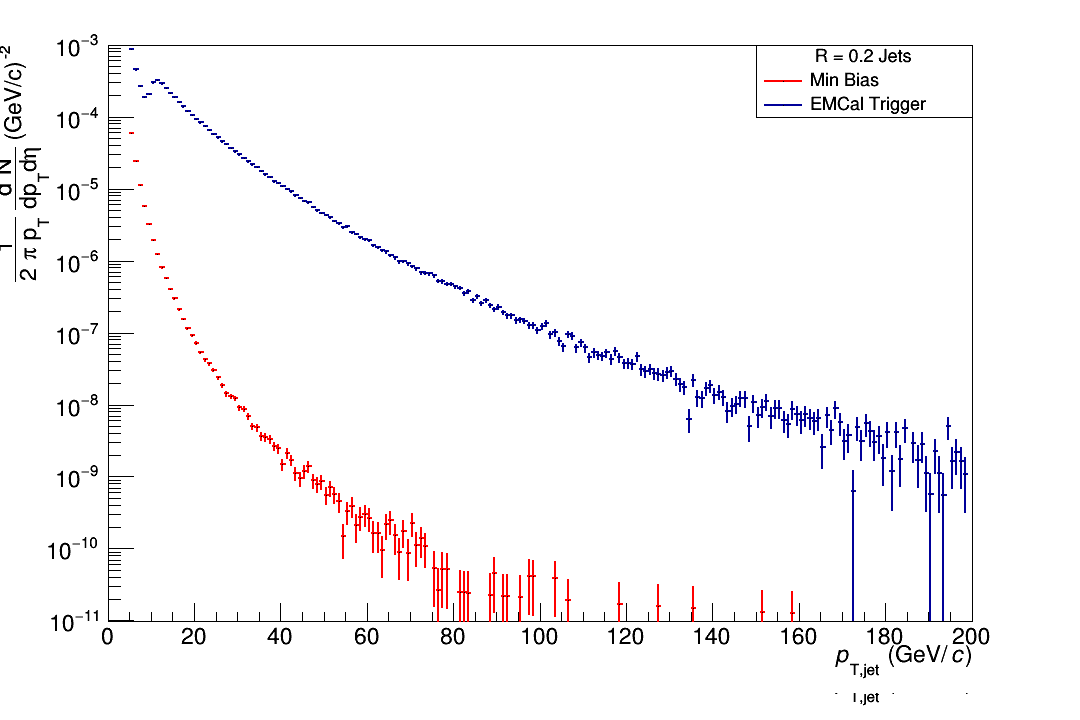
\includegraphics[width=10cm]{RawR02JetSpectra}
\centering
\caption{Raw inclusive R = 0.2 jet spectra from the 8 TeV Min Bias and EMCal triggered data}
\label{fig:rawjetR02}
\end{figure}
\begin{figure}[h]
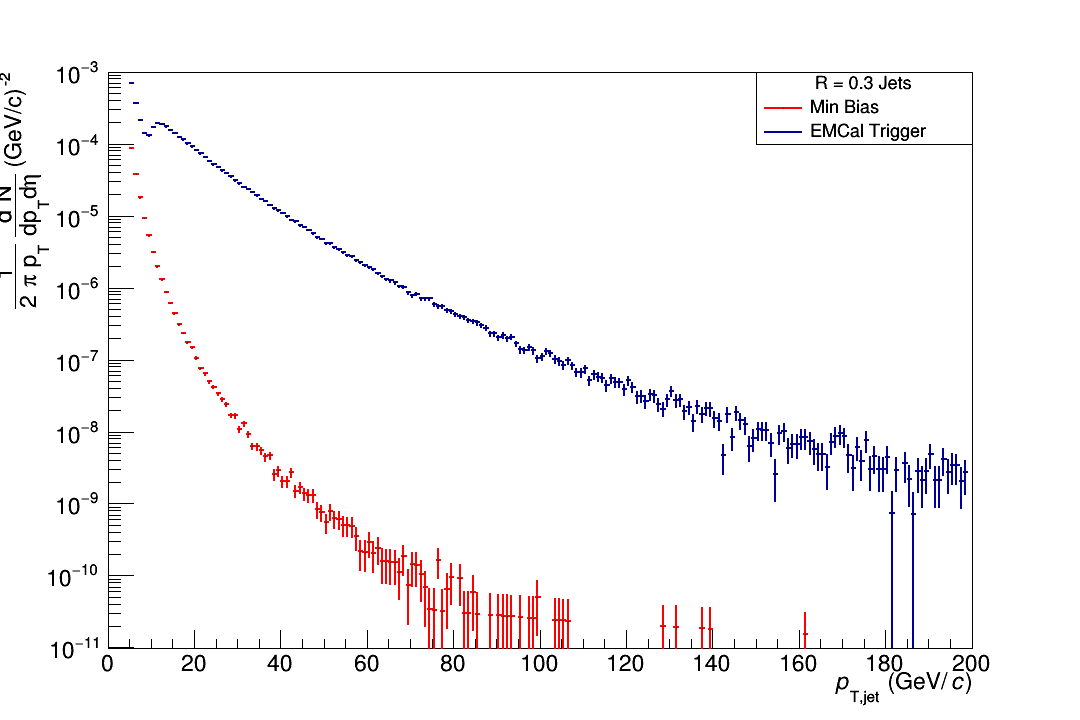
\includegraphics[width=10cm]{RawR03JetSpectra}
\centering
\caption{Raw inclusive R = 0.3 jet spectra from the 8 TeV Min Bias and EMCal triggered data}
\label{fig:rawjetR03}
\end{figure}
\begin{figure}[h]
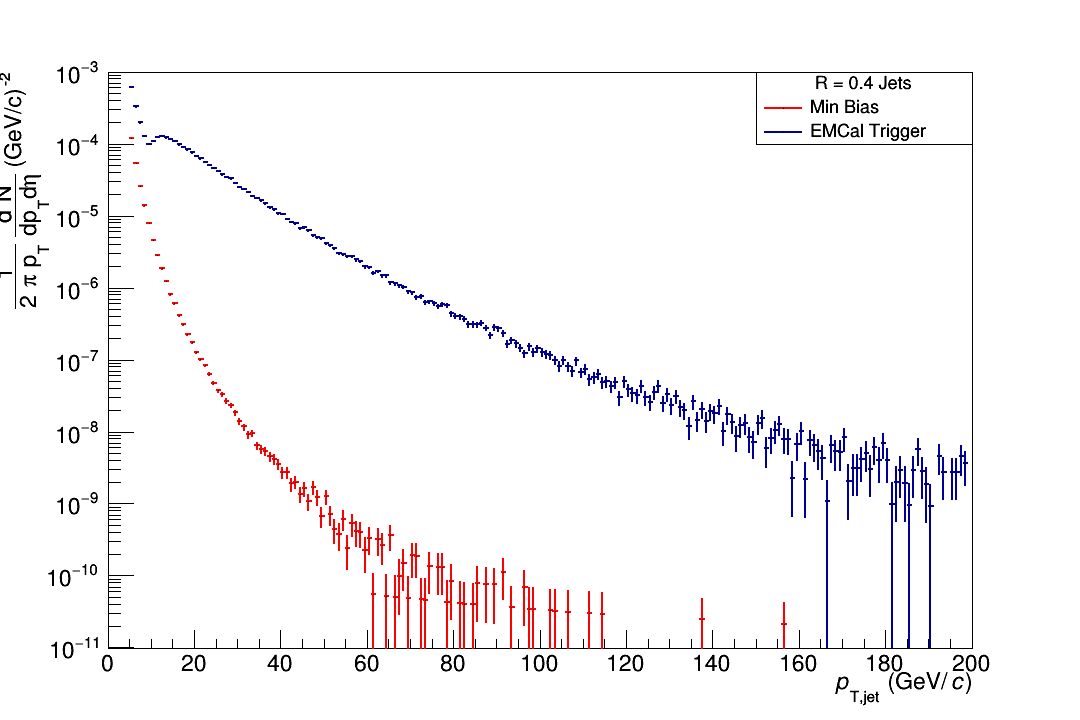
\includegraphics[width=10cm]{RawR04JetSpectra}
\centering
\caption{Raw inclusive R = 0.4 jet spectra from the 8 TeV Min Bias and EMCal triggered data}
\label{fig:rawjetR04}
\end{figure}

\noindent
The next sections of this chapter will discuss the QA implemented to the data, trigger scaling, unfolding, and other corrections 

\section{8 TeV Data Quality}
ALICE is a state-of-the-art experiment with excellent tracking and particle identification capabilities as discussed in Chapter \ref{ch:alice}.  However, just like any real world experiment, it contains a number of inefficiencies and imperfections.  This means that the data collected during the 8 TeV pp collision must be examined and any inaccuracies in the data must be removed before hard physics conclusions may be reached.  Data may be compromised at both the event-level, the experiment erroneously recorded something as an event, or at the constituent-level, one of the subdetectors mismeasured a feature of a particle, and these outliers must be accounted for and removed 

\section{Event Selection}


\begin{figure}[h]
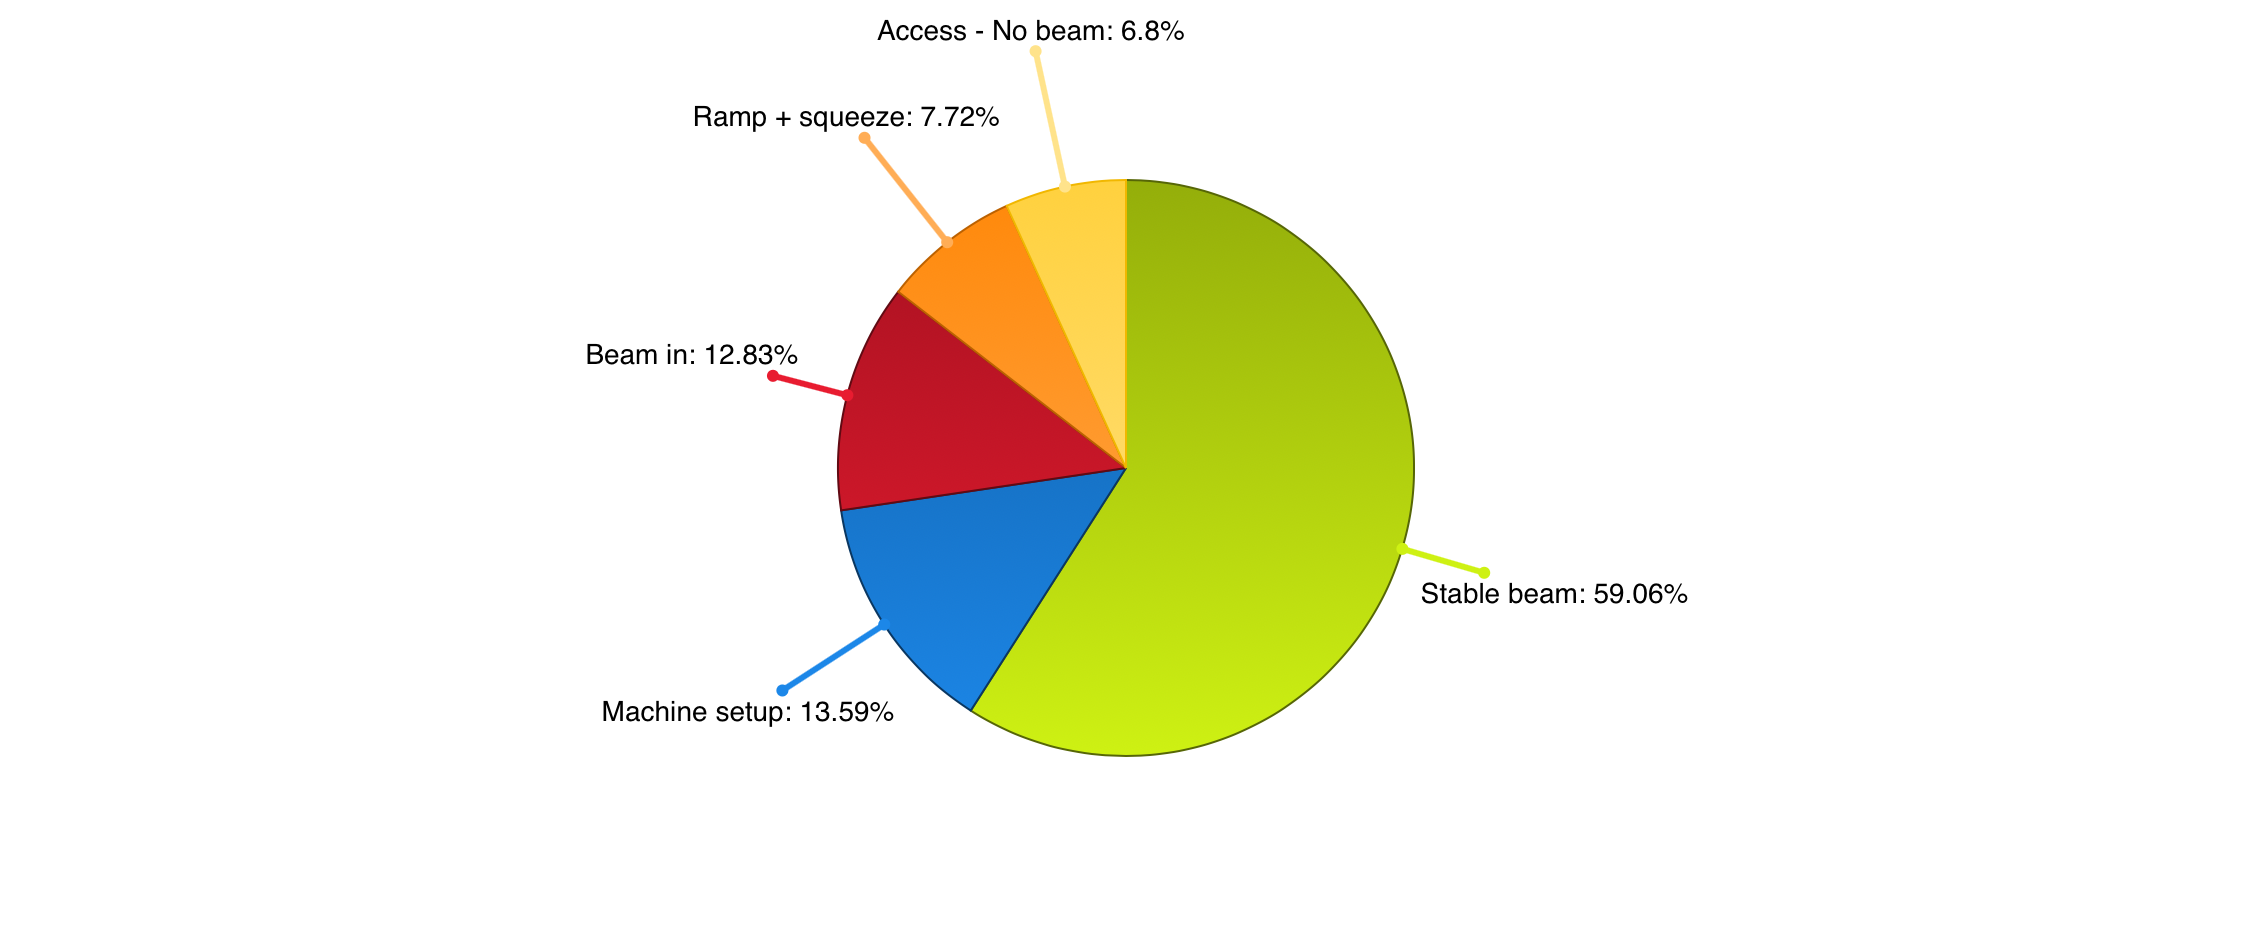
\includegraphics[width=17cm]{8TeVRunefficency}
\centering
\caption{LHC state during the 8 TeV run. }
\label{fig:RunEff}
\end{figure}

During the 8 TeV data collection period approximately 180 million minimum bias events were recorded, as summarized in table \ref{tab:RunSummary}.  These events are separated into periods, which dictate the particular beam and detector configurations during the data taking.The 8 TeV data is broken into 7 periods with approximately 181 million minimum bias events recorded.  This minimum bias sample corresponds to an integrated luminosity, $\mathscr{L}_{int}$, of $8.95 \, pb^{-1}$ during this time period\cite{ALICE-PUBLIC-2017-002}.

\begin{table}[hb]
\label{tab:RunSummary}
\begin{center}
\begin{tabular}[b]{|c|c|c|}
	\hline
	Period & \# of runs & \# of Min Bias events \\ \hline
	LHC12c & 89 & $\sim \,$24 M \\ \hline
	LHC12d & 140 & $\sim \,$62 M \\ \hline
	LHC12e & 5 & $\sim \,$2 M \\ \hline
	LHC12f & 56 & $\sim \,$15 M \\ \hline
	LHC12g & 8 & $\sim \,$0.4 M \\ \hline
	LHC12h & 159 & $\sim \,$75 M \\ \hline
	LHC12i & 40 & $\sim \,$3 M \\ \hline
	Total & 497 & $\sim \,$181 M \\ \hline

\end{tabular}
\end{center}
\caption{2012 8 TeV data taking period.}
\end{table}

Approximately, 15\% of the data sampled is unusable due to malfunctions in TPC chambers, EMCal super modules, the electronics for the EMCal or TPC,.  LHC12a,b triggered data is not used in this analysis due to the trigger threshold being varied from the other periods.  

\subsection{Monte Carlo Anchored Data}
The ALICE Collaboration produced two Monte Carlo data sets anchored to the detector performance during the 8 TeV run.  LHC15l2a1 is a PYTHIA anchored data set that consisted of about 17 million Min Bias triggered events and LHC15l2a2 is a PHOjet anchored data set consisting of about 21 million Min Bias triggered Events.  Neither of these data driven Monte Carlos modeled the EMCal triggers.

\subsection{General Event Section Criteria}
For an event to be selected into a physics analysis it must pass a number of quality control tests.  For example, the LHC must have be in a state of stable beams, cosmic rays must be excluded by only accepting tracks that originate from a vertex inside the detector, and the relevant detectors for a given analysis must be functioning as intended.  Event selection and QA is implemented via a centralized class, AliEventCuts, within the AliRoot framework.  This class contains a number of corrections including:

\begin{itemize}
  \item The event has a primary vertex reconstructed.
  \item The primary vertex occurs within a 10 cm window of the primary interaction point.
  \item The vertex resolution must be below 0.25 cm.
  \item The event passes basic pile-up checks based on the V0 and T0 signals.
\end{itemize}

\noindent
A summary of the rejection reasons at the event level is summarized in Figure \ref{fig:eventqa}.

\begin{figure}[h]
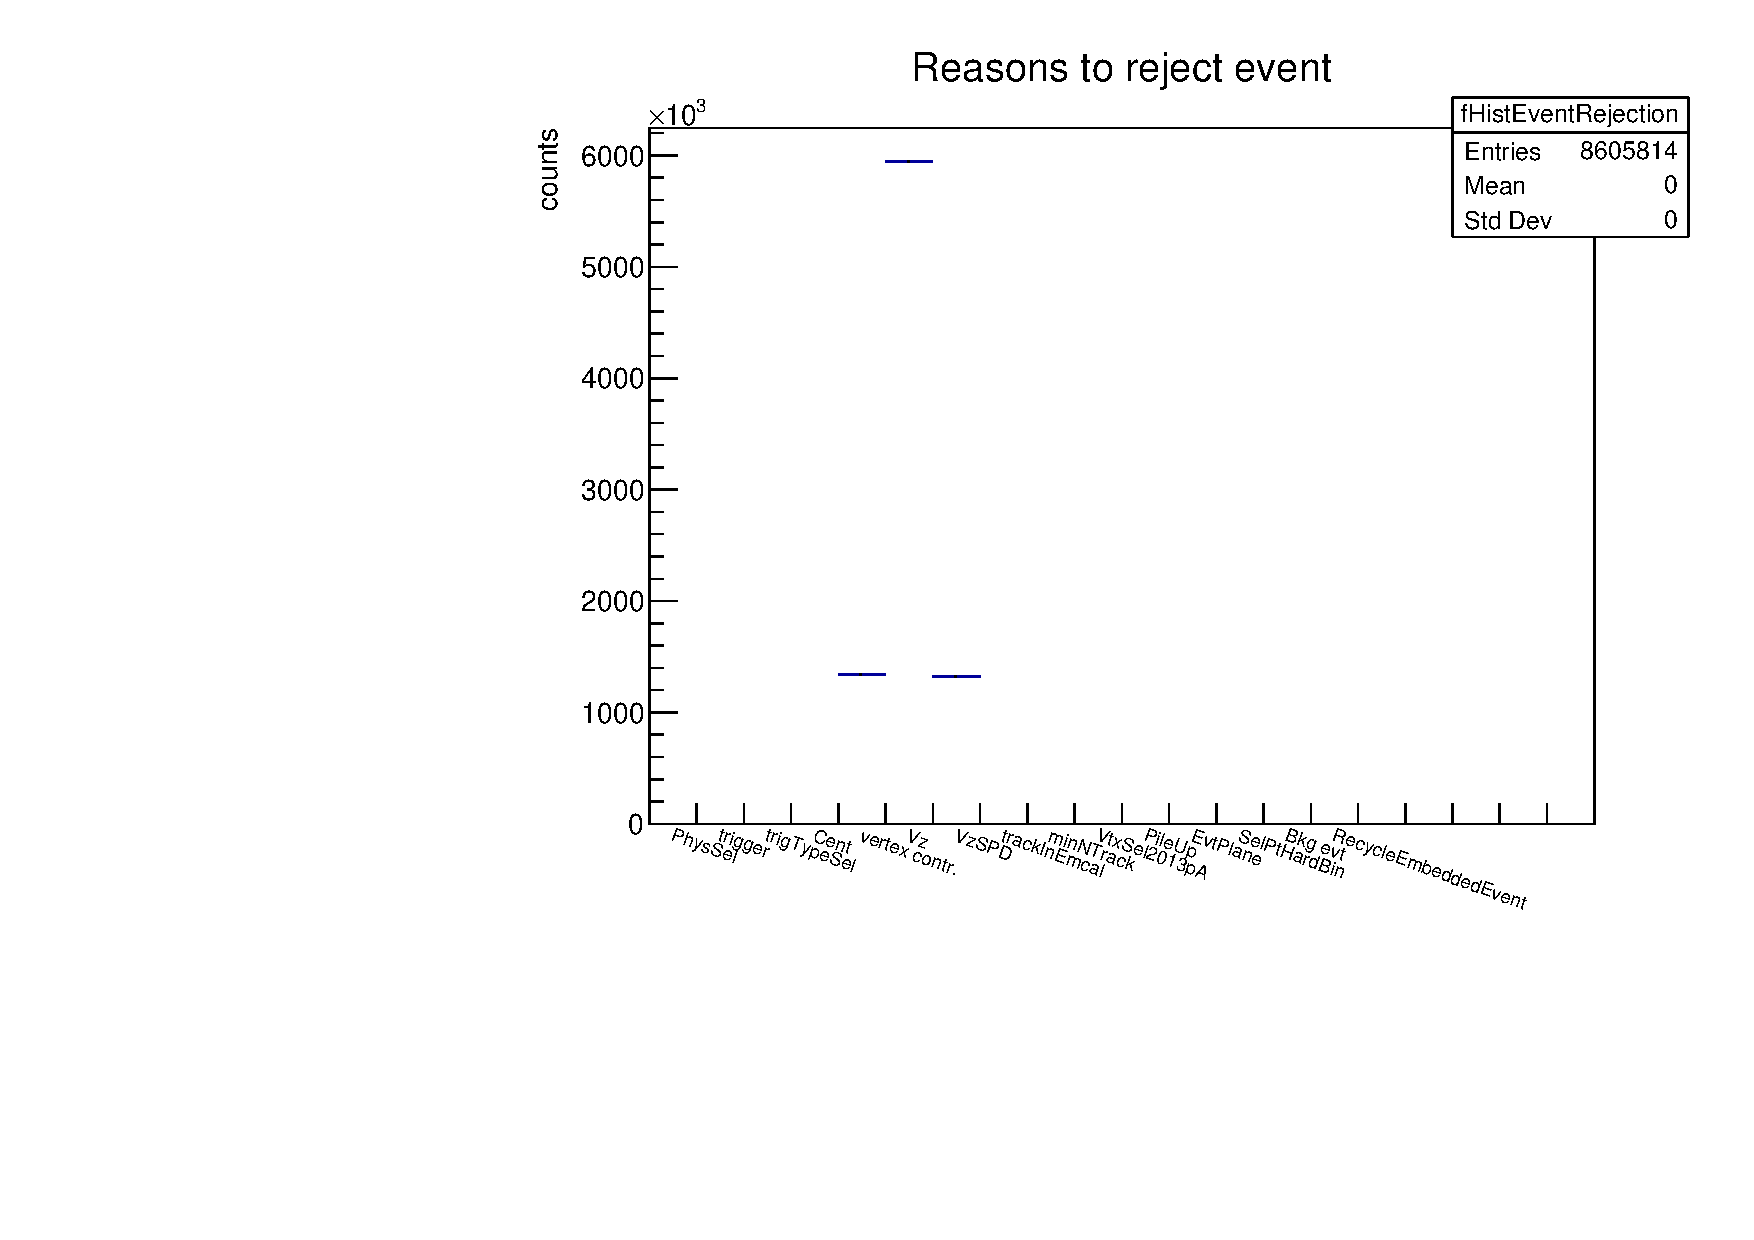
\includegraphics[width=10cm]{RejectionReasons}
\centering
\caption{Min Bias event rejection summary.}
\label{fig:eventqa}
\end{figure}

\begin{figure}[h]
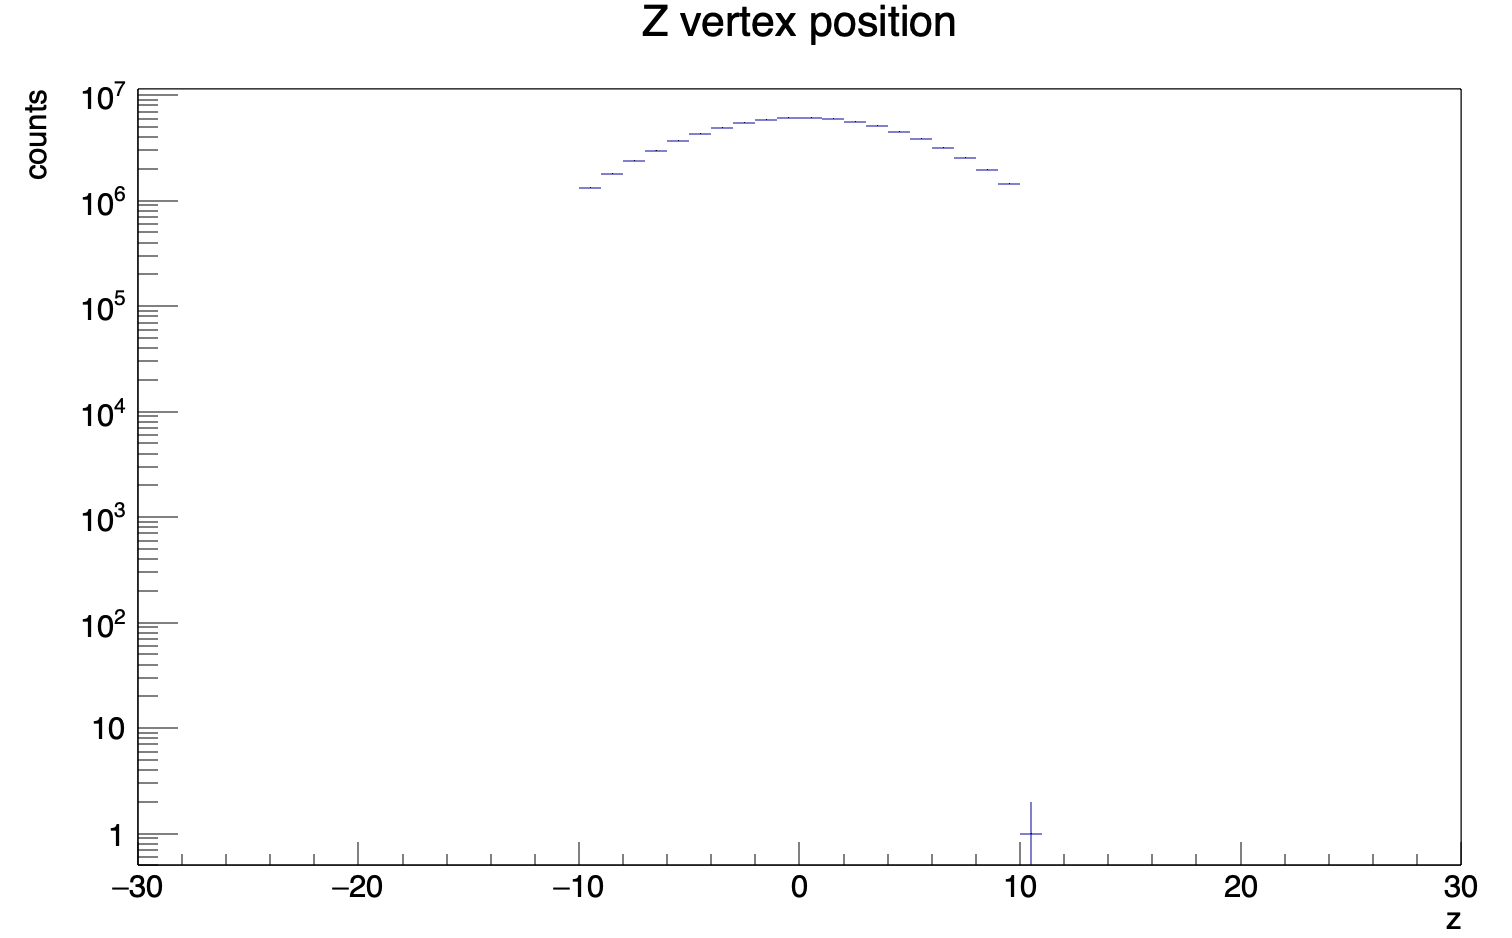
\includegraphics[width=10cm]{zvertex}
\centering
\caption{Vertex displacement from primary interaction point for accepted Min Bias events.}
\label{fig:vertrec}
\end{figure}

\noindent 
Figure \ref{fig:vertrec} shows the reconstructed vertex for the accepted Min Bias events.  We see that the vertex distribution peaks at the primary interaction point as expected.  It should also be noted that a similar set of event QA was implemented to the EMCal triggered data \textit{(not shown)} and that the results were consistant with the Min Bias data.

\section{EMCal Cluster Selection}
Corrections are performed on EMCal cells including; removing hot and dead towers (bad channels) based on the average occupancy and energy of the towers, calibrations to cell timing caused by the physical layout of the EMCal (such as differences in cabling length), and a energy calibration is implemented based on the $\pi^{0}$ mass.  After these corrections are applied to the towers are grouped together into clusters using the v2 algorithm.  The v2 algorithm has a minimum tower seed, $E_{seed} = \,$ 300 MeV, after which all adjacent towers with a minimum energy, $E_{cell} \geq \,$ 100 MeV, are iteratively added until a local minimum is reached.  The cluster energy is the sum of the seed and grouped neighbor tower energies.   

\begin{figure}[h]
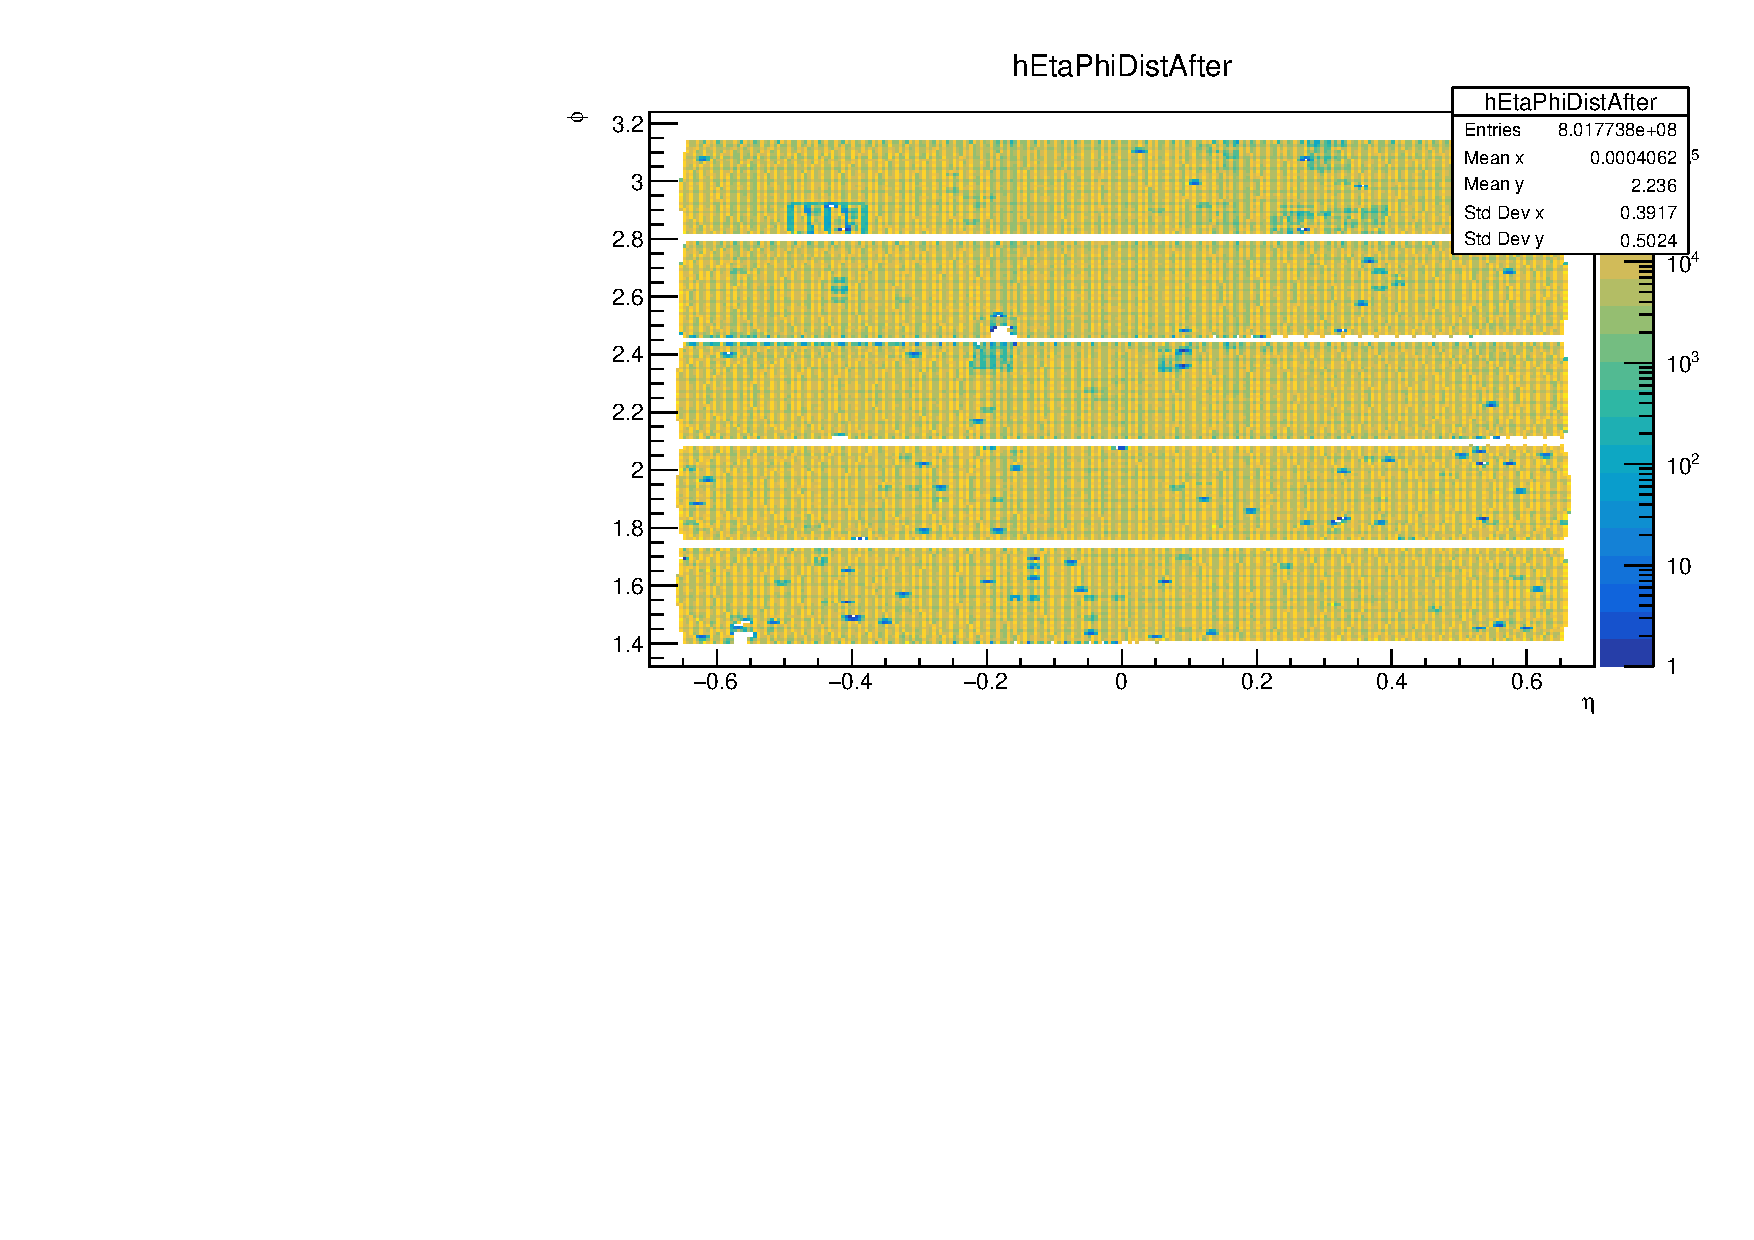
\includegraphics[width=14cm]{BadChannelMap}
\centering
\caption{EMCal cell occupancy after bad channels removed.}
\label{fig:badchannel}
\end{figure}


\noindent
Figure \ref{fig:badchannel} shows the bad channel map after removing bad towers, the $\phi$ distribution is segmented into 5 parts representing the five super modules of the EMCal.  After the cells are clustered together the clusters are corrected for exotics.  This correction is performed by cutting all clusters with a $F_{cross} \geq \,$ 0.97, where

\begin{equation}
F_{cross} = 1 - \frac{ E_{cross} }{ E_{cell} },
\label{eq:Fcross}
\end{equation}

\noindent
$E_{cross}$ is the sum of the four cells sharing a full edge with the leading cell.  The main source of exotic clusters in the EMCal is due to a hadron hitting the Avalanche Photodiode (APD) in a tower.  This will concentrate the energy of the cluster into a single tower while the adjacent towers will contain only a small fraction of the cluster energy.  These clusters are removed before jet finding occurs as they are not part of the jet energy.

The EMCal is optimized to measure the energy of electrons and photons as they tend to fully shower inside the EMCal structure.  Hadrons are detected by the EMCal but will only shower a fraction of their intrinsic energy.  A hadronic correction is performed in order to account for this missing energy due to the partial hadron shower.  Charged tracks from the outer layer of the TPC are propagated to the EMCal and the centroids of the clusters and tracks are matched together.  Figure \ref{fig:EMChadetaphi} shows the distance between the centroid of a cluster in the EMCal to the nearest track propageted from the TPC.  Hadrons are identified by requiring the matched distance to be, $\sqrt{ \Delta\phi^{2} + \Delta\eta^{2} } \leq \,$ 0.015, which is within one EMCal tower distance.

\begin{figure}[h]
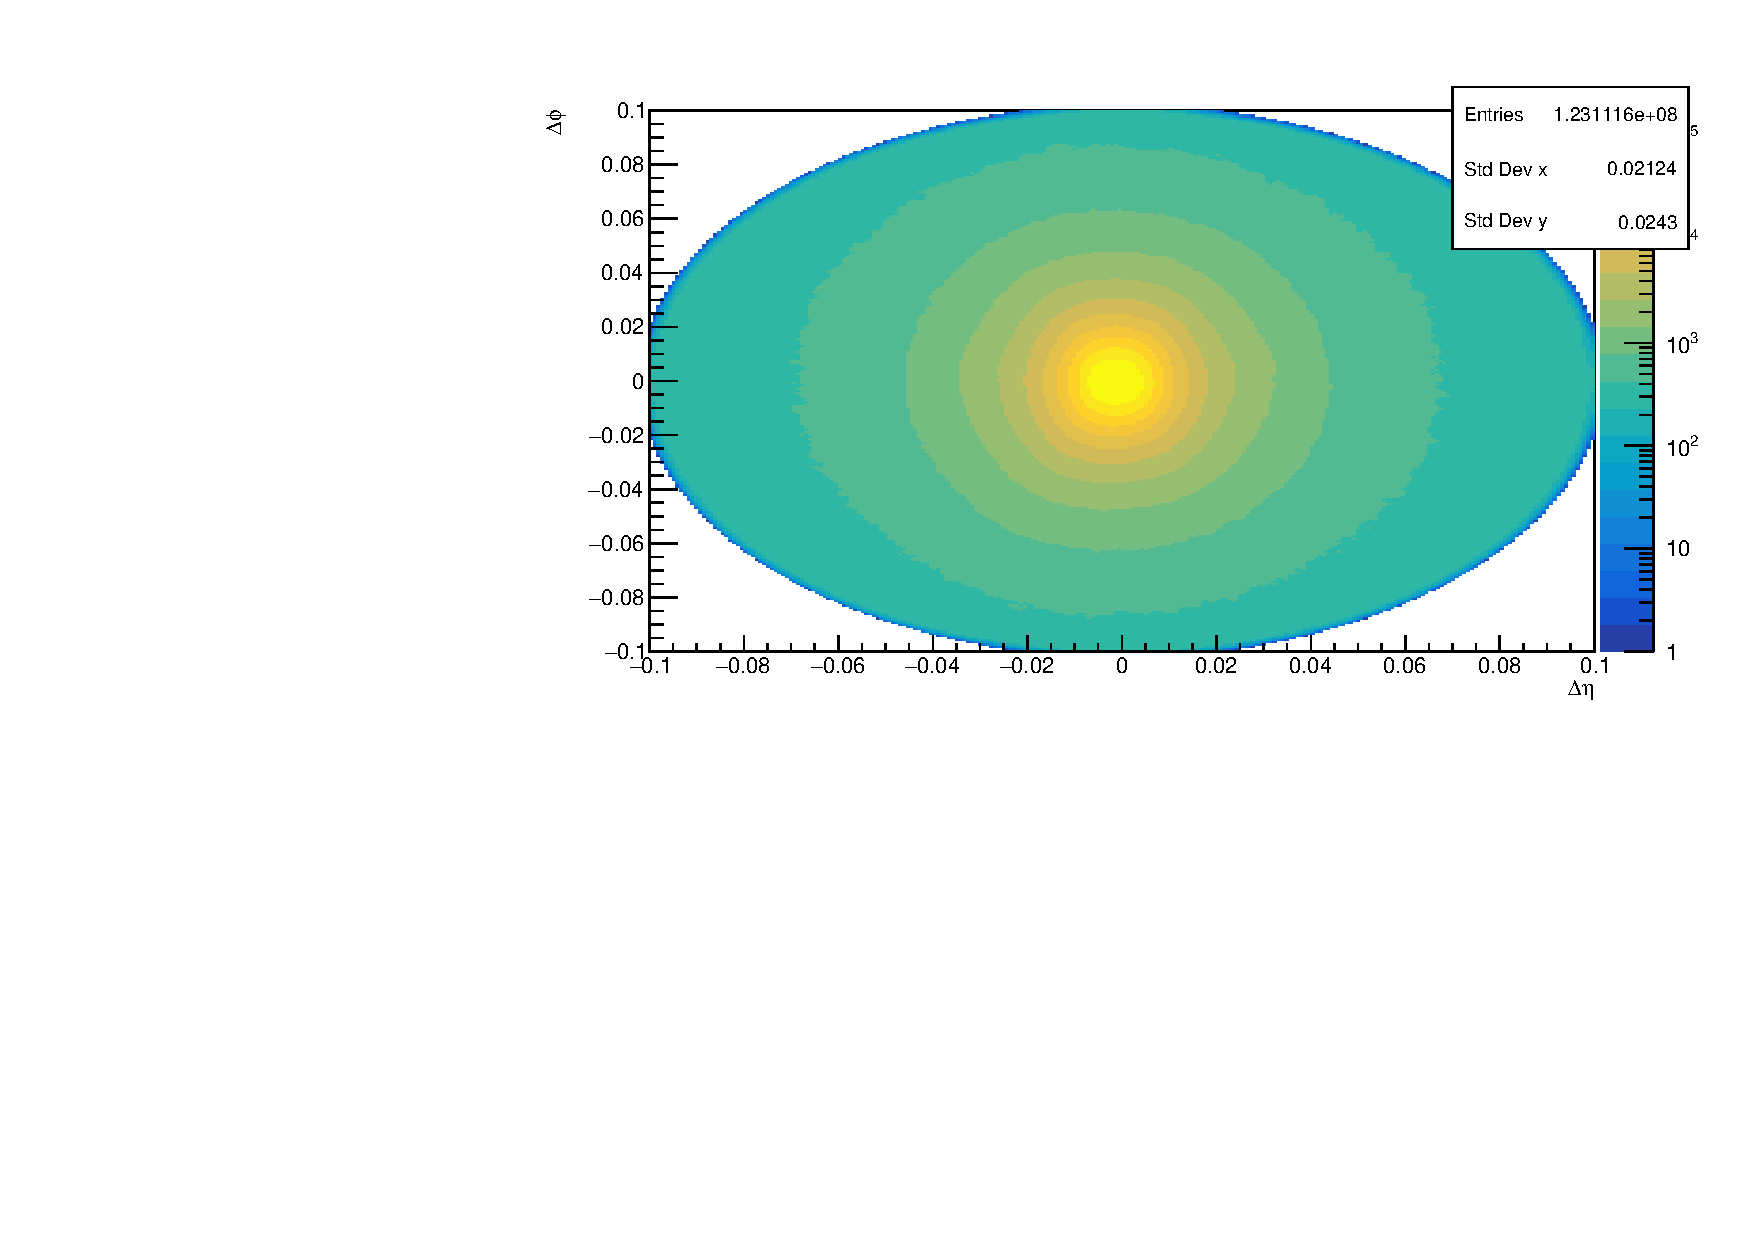
\includegraphics[width=12cm]{hadronetaphi}
\centering
\caption{Matched track-cluster distance.}
\label{fig:EMChadetaphi}
\end{figure}

\noindent
Corrections for the double counting from hadrons is based on correcting the EMCal cluster energy by a weight function,

\begin{equation}
E_{corr} = E_{clust} - f_{sub} \times \sum p ,
\label{eq:HadCorr}
\end{equation}

\noindent
where $\sum p$ is the magnitude of the 3-mommentum of the hadron and $f_{sub} = 1$ is the nominal value for the weight.  If $E_{corr} \leq 0$ the cluster is removed, this may be caused by cluster pile-up and only accounts for a small fraction of the clusters.  In order for a cluster to be accepted $E_{corr} \geq \,$ 300 MeV was required.  The 300 MeV threshold is required because a minimum ionizing particle (MIP) will on average deposit 280 MeV in the EMCal.  

A final cut was performed on the cluster time.  
\begin{figure}[h]
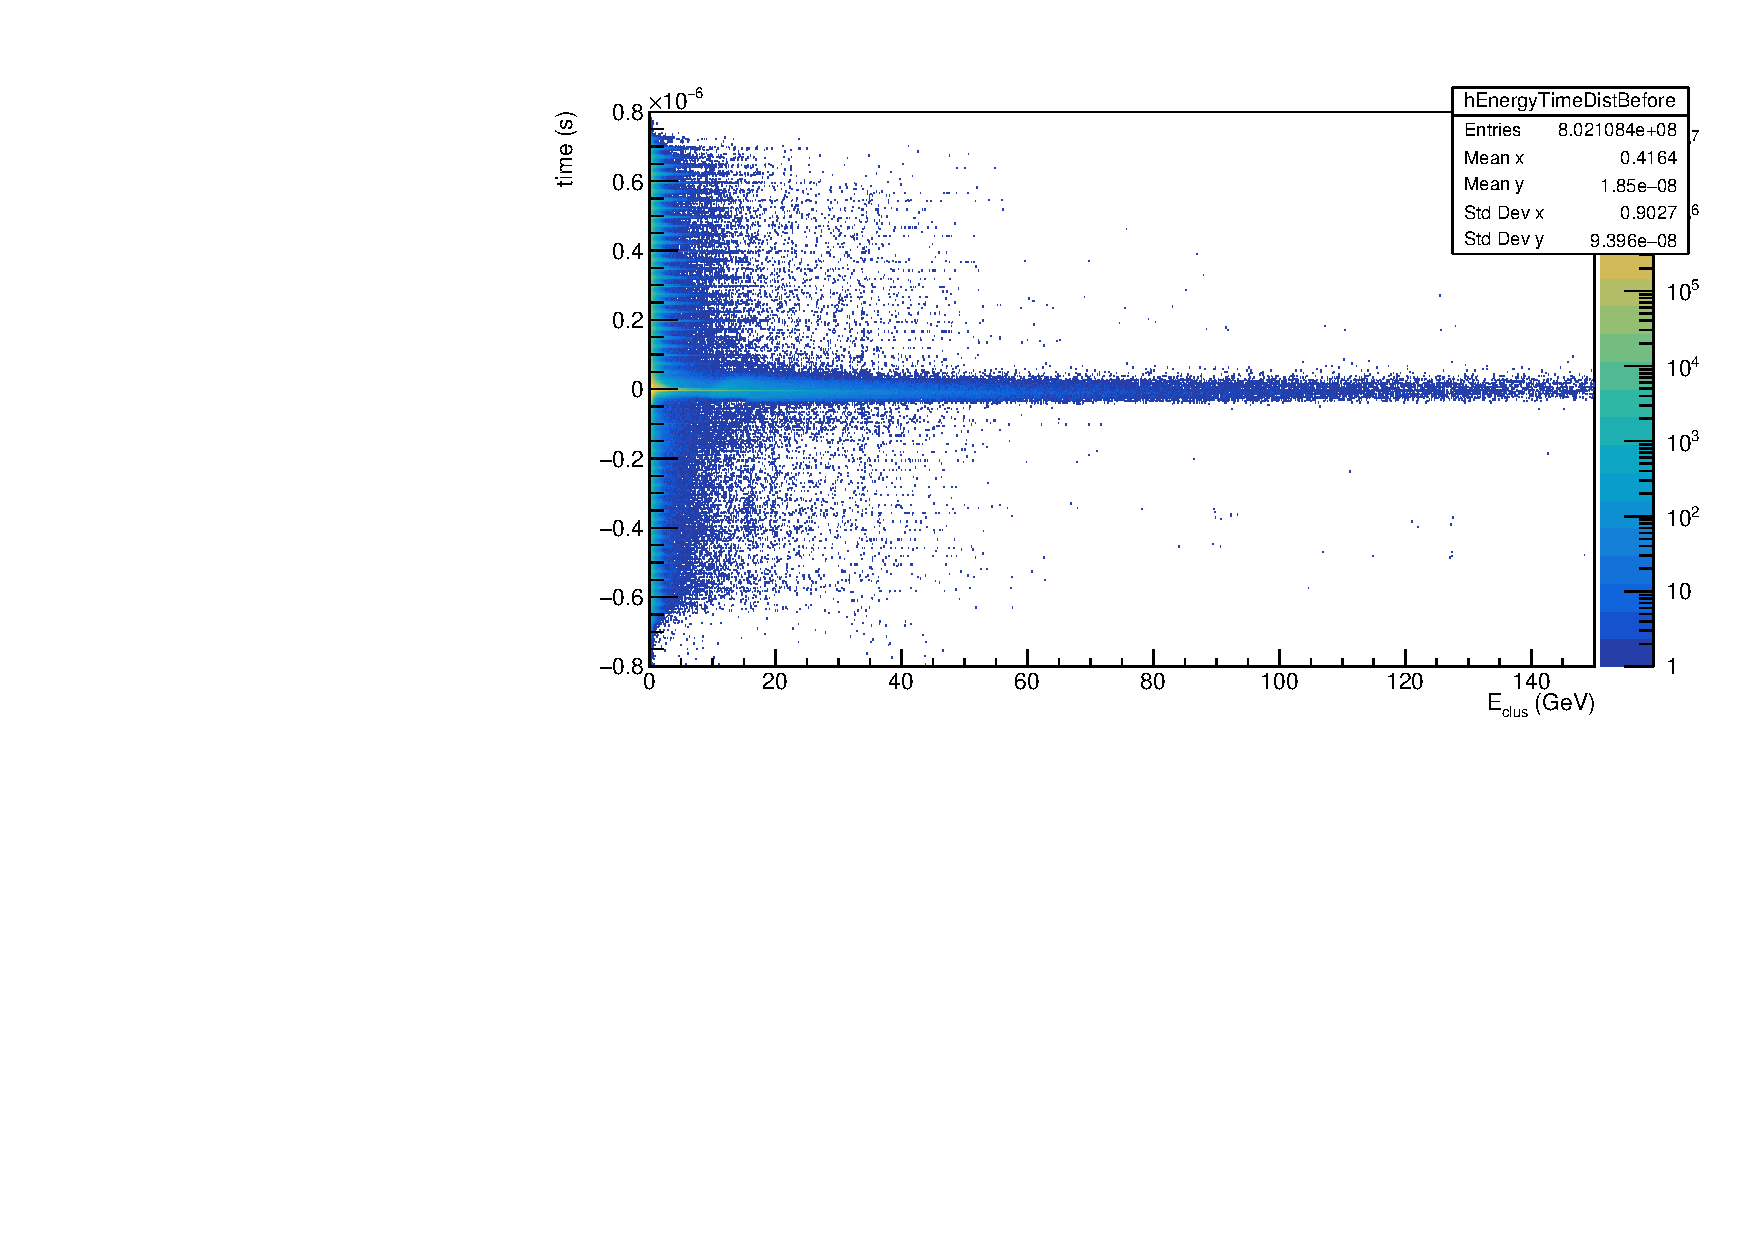
\includegraphics[width=12cm]{timming}
\centering
\caption{EMCal cluster time distribution before cuts.}
\label{fig:EMCaltime}
\end{figure}

\noindent
Cutting on the cluster time is done in order to readout only the particles created from an event and to limit the contaimination due to slower particles from previous events.  The main source of the slow moving particles are neutrons and $K_{L}^{0}$ and this analysis limits cluster time to $t_{clus} \epsilon \,$ [-50 ns, 100 ns].


\begin{figure}[h]
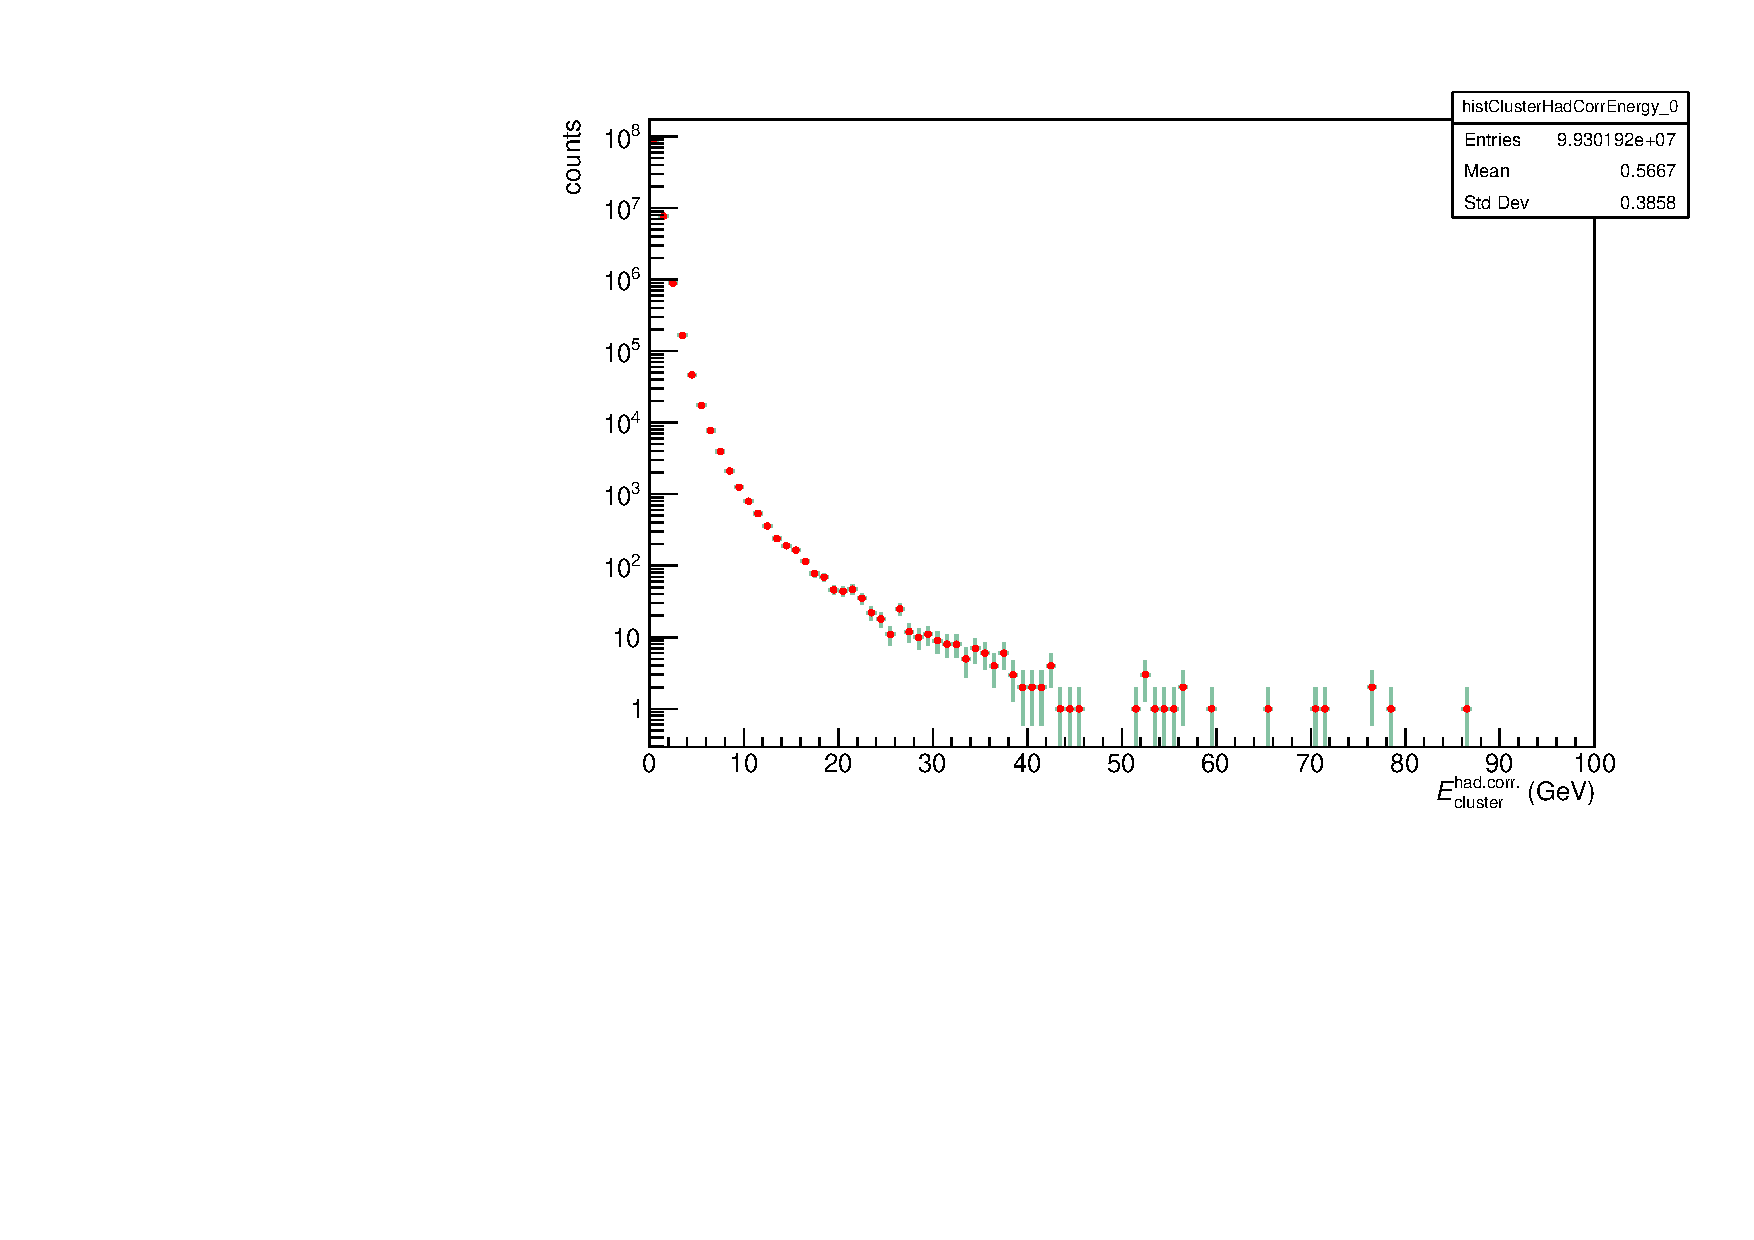
\includegraphics[width=12cm]{Eclusfinal}
\centering
\caption{Corrected EMCal cluster yield.}
\label{fig:EMCalfinal}
\end{figure}
\newpage

Figure {fig:EMCalfinal} shows the final cluster energy distribution with all the cuts and corrections previously discussed applied and makes up the set of clusters over which the jet finding was performed.  The same cuts and QA was applied to the EMCal triggered data.
 
\section{TPC Track Selection}

Tracks are reconstructed in the TPC using a Kalman filtering which helps alleviate any corrections needed due to multiple scatterings, dead sectors, etc.  Jet finding was performed using `hybrid' tracks.  Hybrid tracks consist of two track sets the first being all the tracks with at least one hit in the SPD (Global) and the second set being all tracks that can be costrained to the primary vertex (Complimentary).  For this analysis, the minimal $p_{T, track}$ is 150 MeV/c and the track must be constrained to: - 0.9 $\leq \eta \leq$ 0.9 and 0 $\leq \phi \leq$ 2$\pi$, shown in Figure \ref{fig:Hybridtracketaphi}.  The spatial distributions of the hybrid tracks remain relatively flat as expected in the 8 TeV data set.

\begin{figure}%
    \centering
    \subfloat[Hybrid Track $\eta$]{{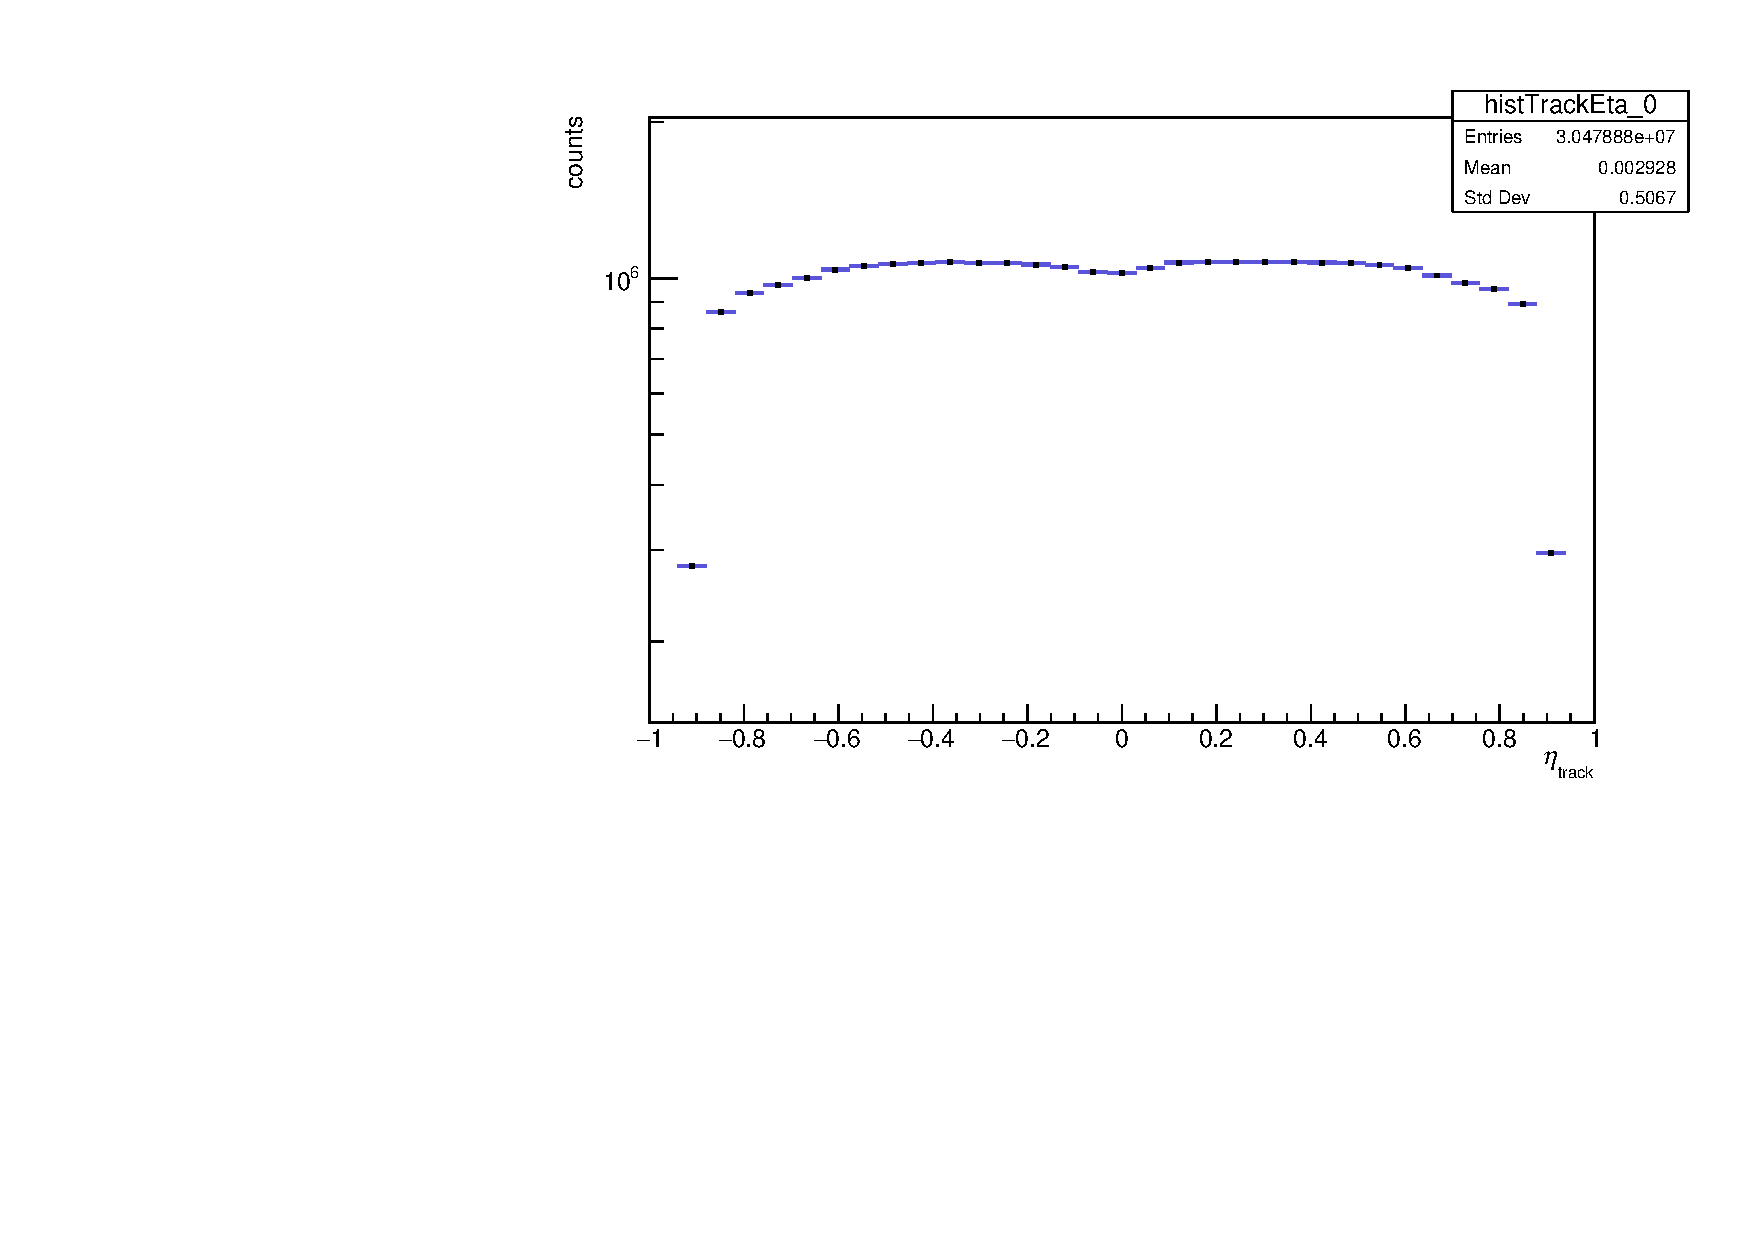
\includegraphics[width=5cm]{tracketa} }}%
    \qquad
    \subfloat[Hybrid Track $\phi$]{{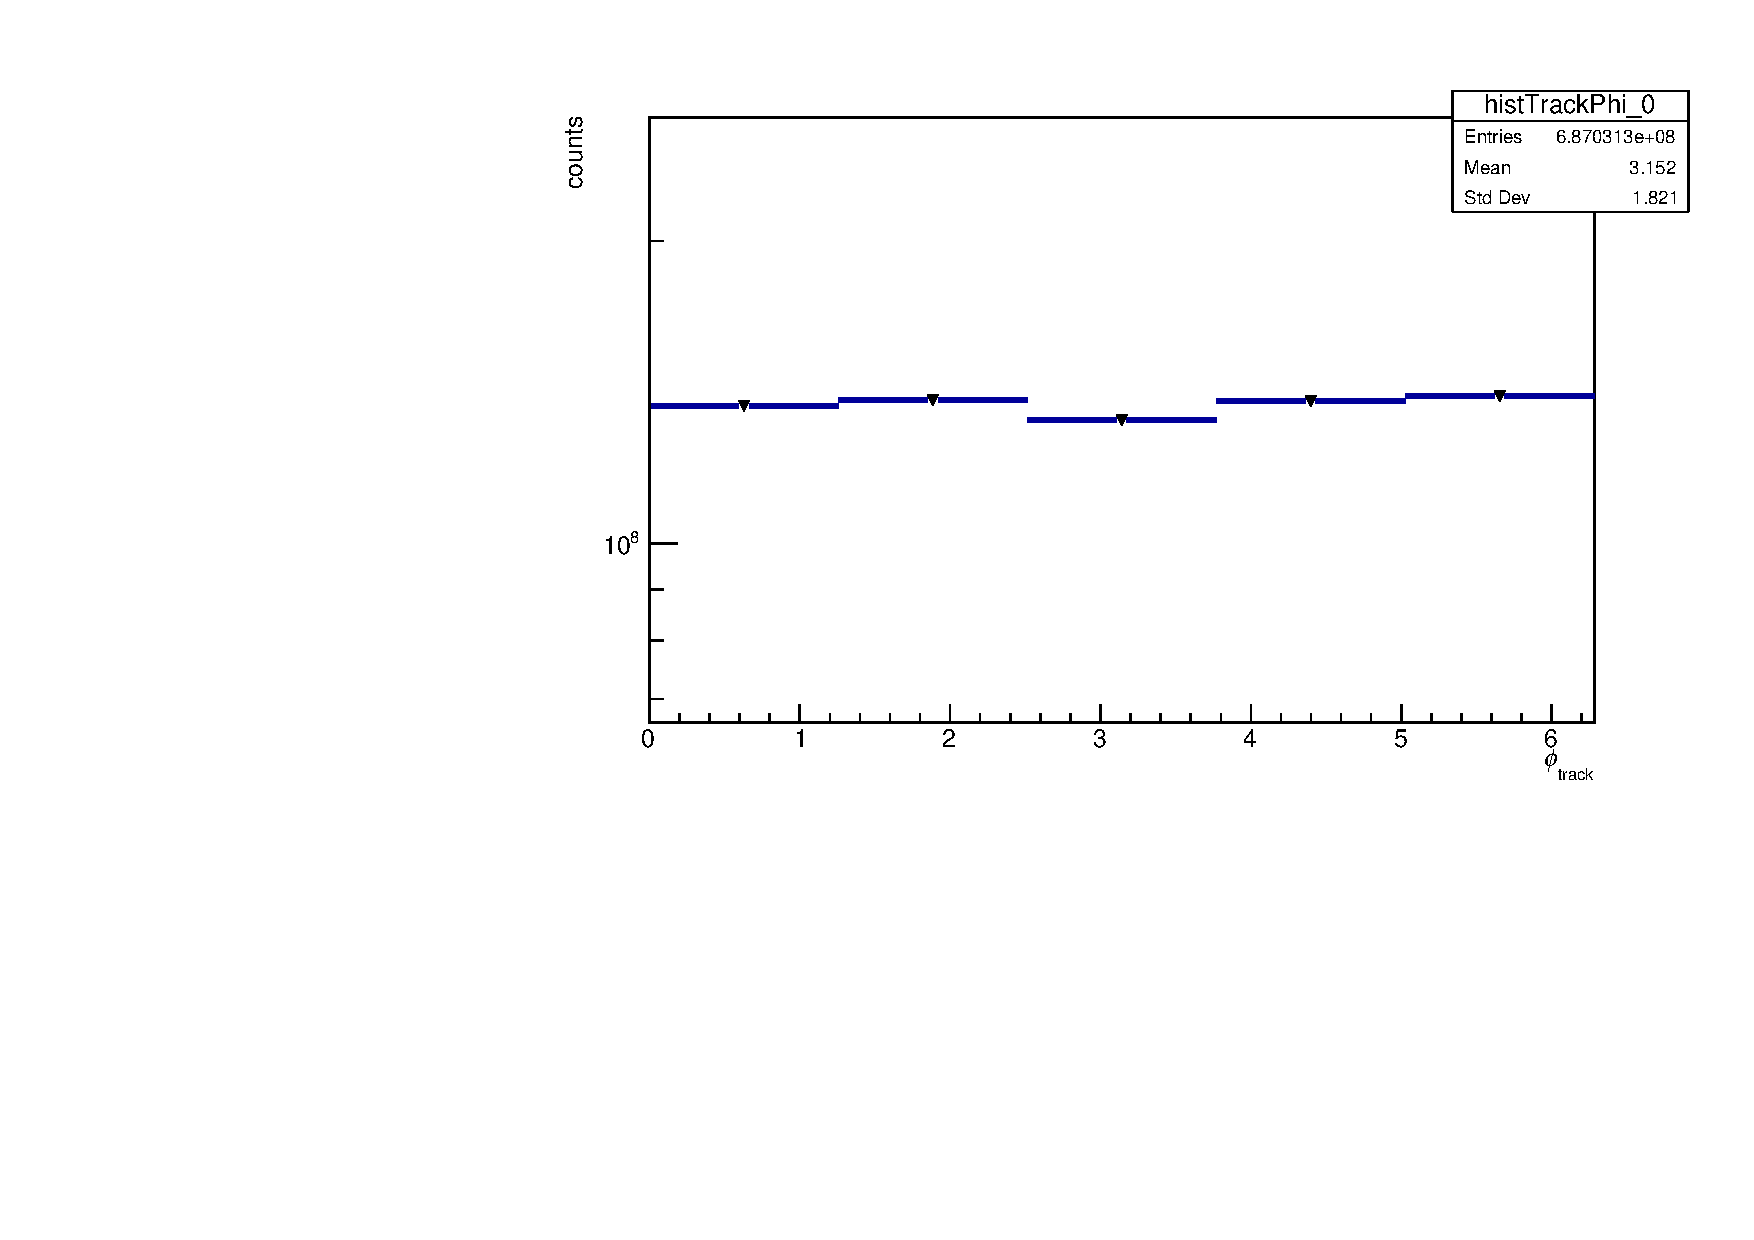
\includegraphics[width=5cm]{trackphi} }}%
    \caption{Hybrid Track $\eta$ and $\phi$ yields.}%
    \label{fig:Hybridtracketaphi}%
\end{figure}

\noindent
The quality of the jet $p_{T}$ resolution was maintained by only accepting jets into the jet finder with a resolution below 1\%, Figure \ref{fig:trackresolution}, and this $p_{T}$ distribution may be seen in Figure \ref{fig:hybtrackpt}.

\begin{figure}[h]
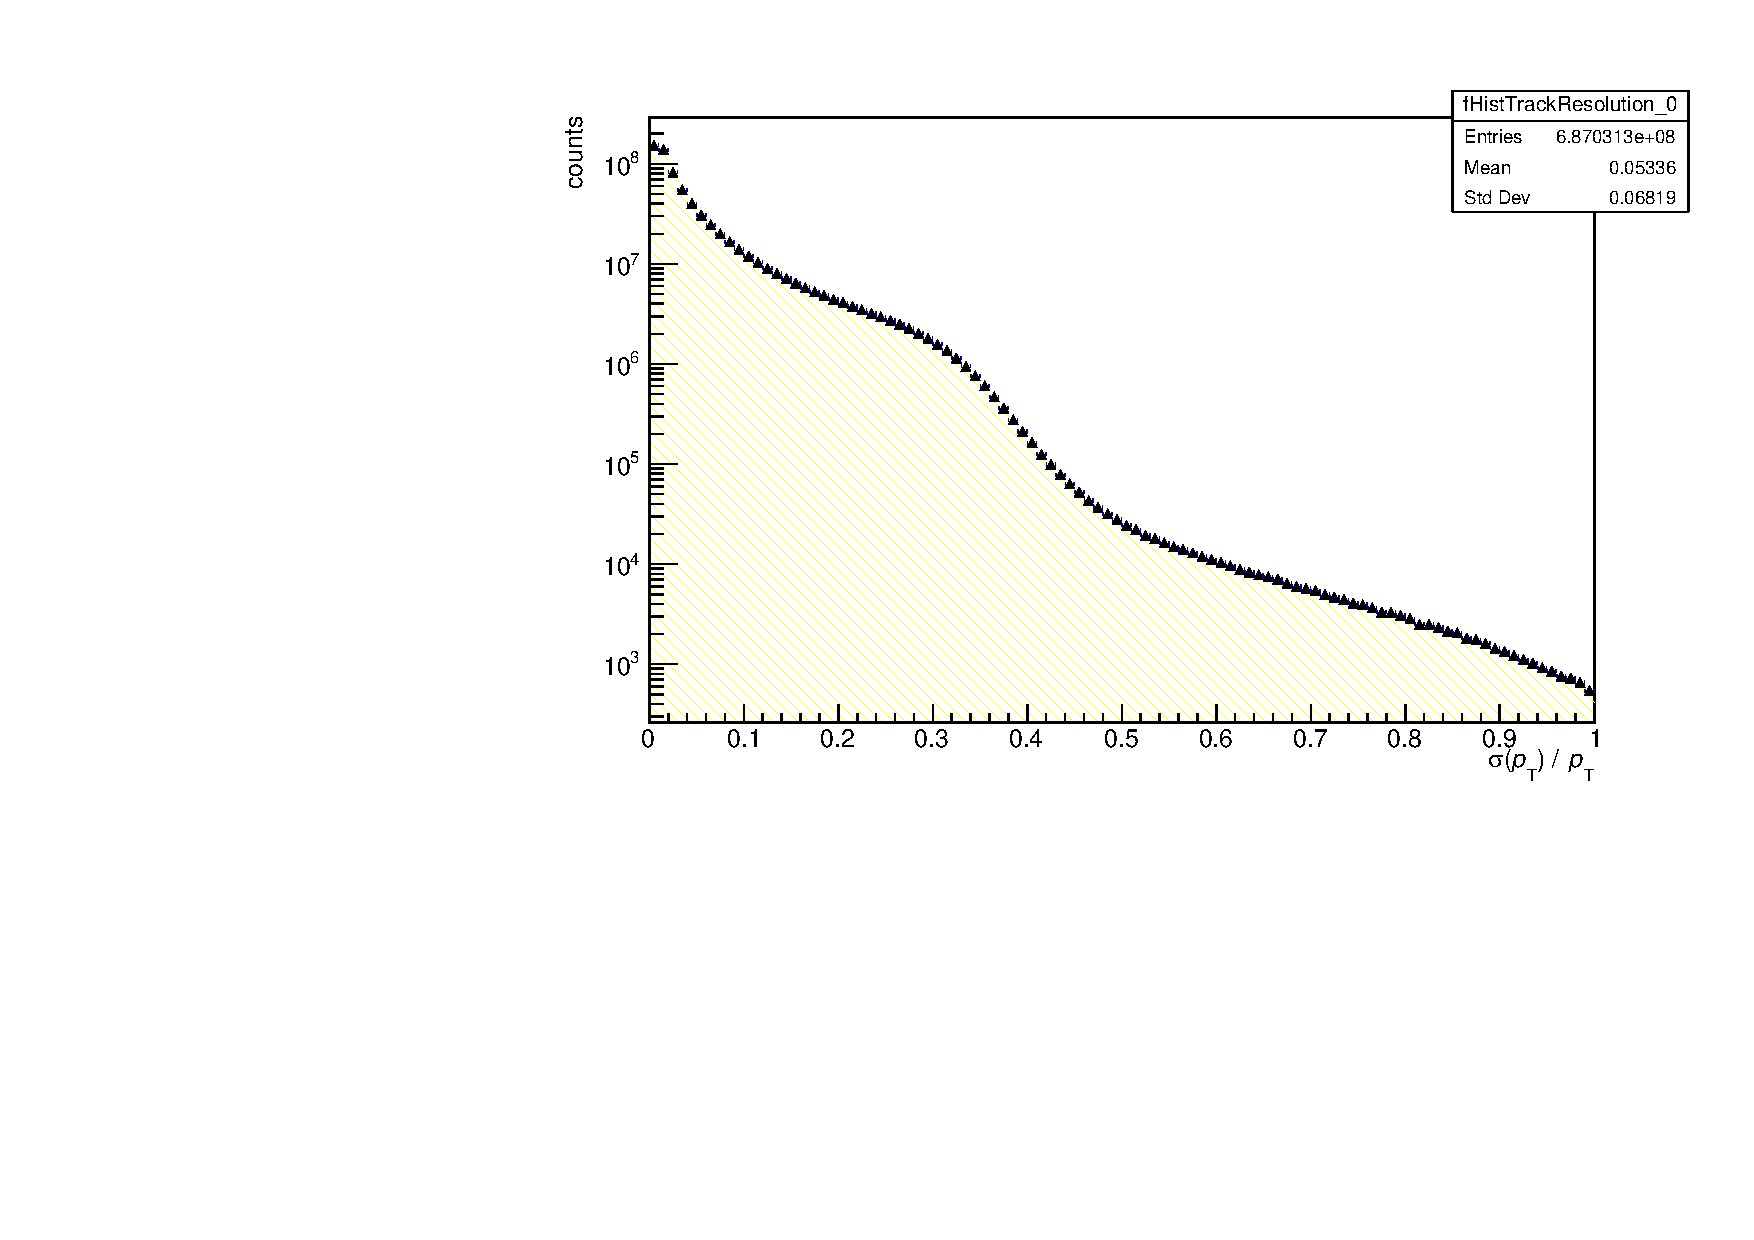
\includegraphics[width=10cm]{trackresolution}
\centering
\caption{Accepted hybrid track resolution.}
\label{fig:trackresolution}
\end{figure}

\begin{figure}[h]
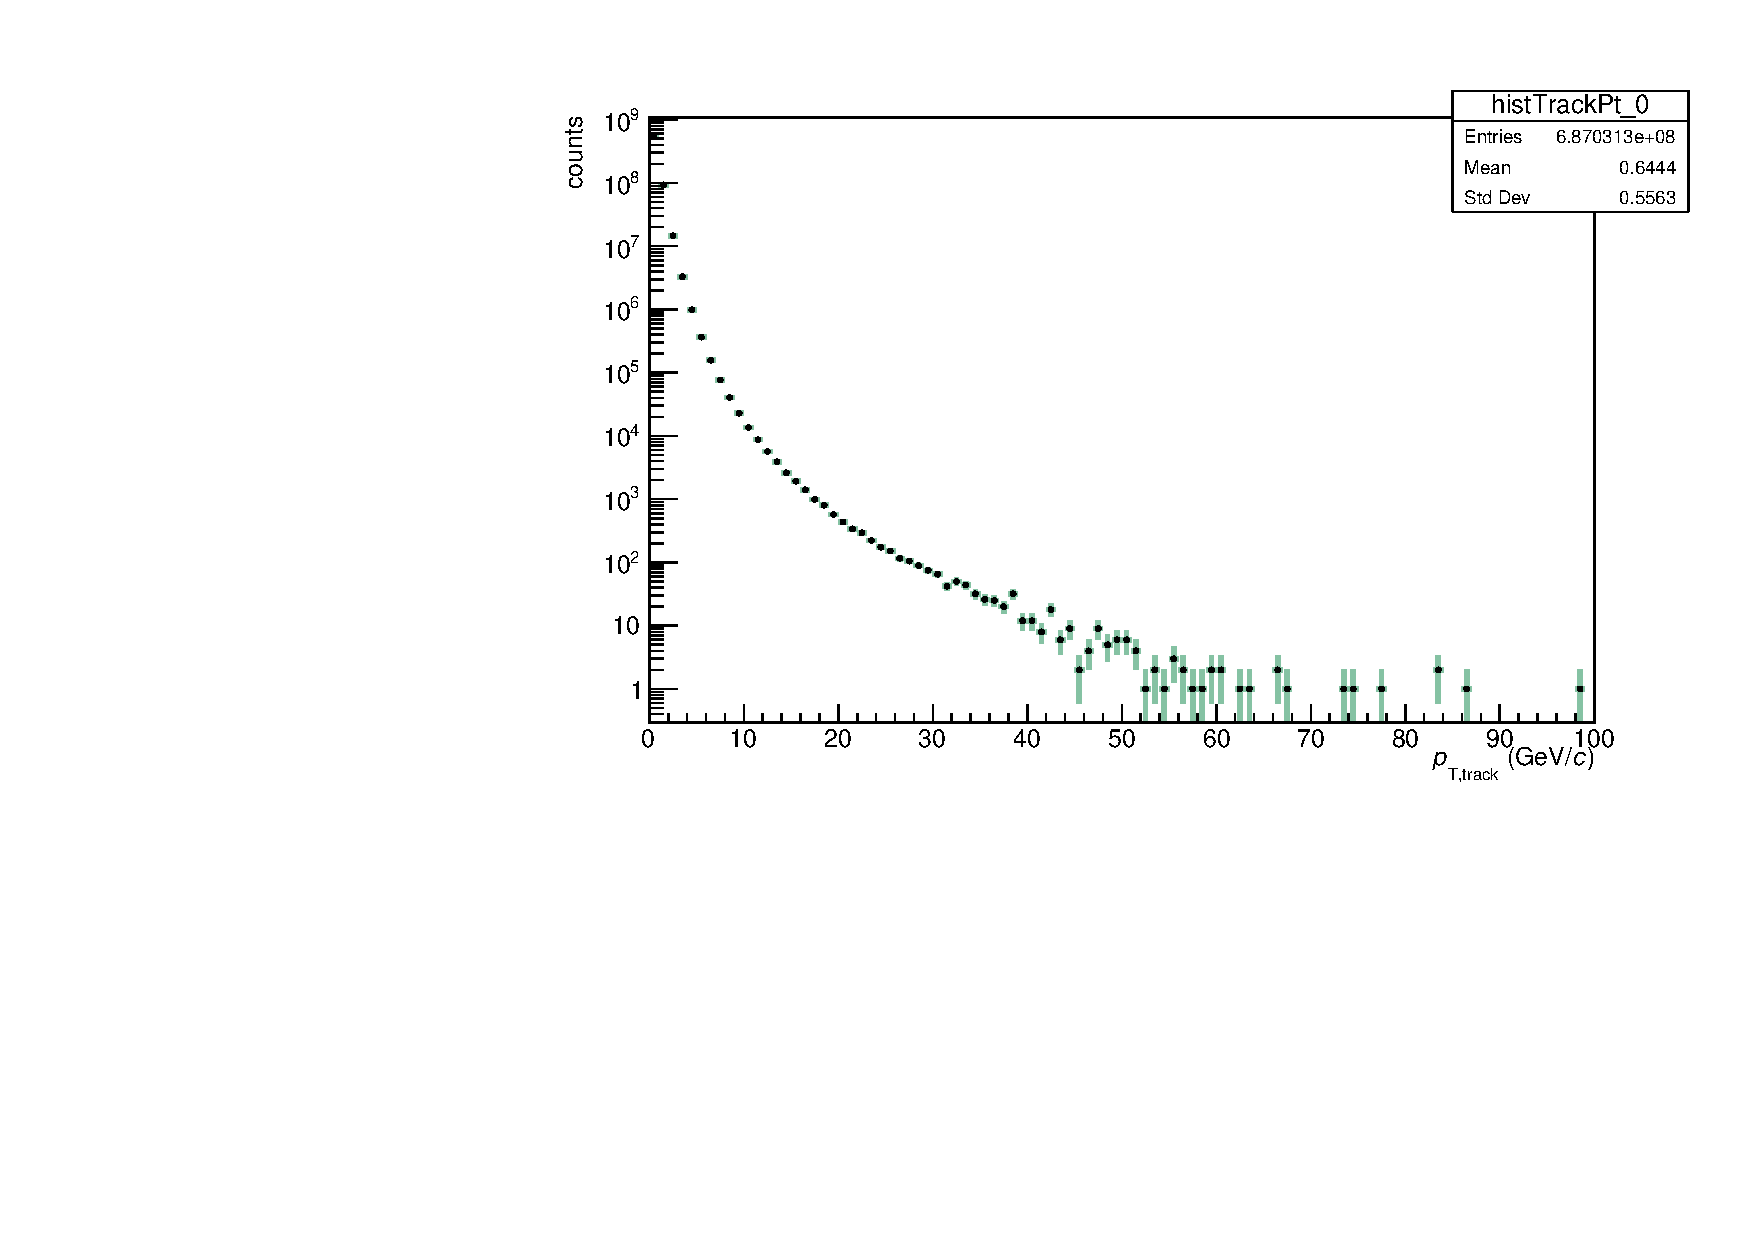
\includegraphics[width=10cm]{trackpt}
\centering
\caption{Accepted track $p_{T}$ yield.}
\label{fig:hybtrackpt}
\end{figure}

\noindent
These cuts followed a number of previous track cuts seen in a number of jet results published from ALICE\cite{Acharya:2018eat}.
\newpage
\section{Jet Selection}

Accepted tracks and clusters are feed into the anti-kt jet reconstruction algorithm to reconstruct inclusive jets.  A minimum threshold of 5 GeV was used to reconstruct a jet in this analysis.  A high-$p_{T}$ track threshold of 100 GeV is placed on the reconstructed jets.  This is motivated by the degradation of the momentum resolution above that energy range.  In addition a cut was applied that a jet must be composed of at least one constituent, Figure \ref{fig:JetPt} and \ref{fig:JetConst}.

\begin{figure}[h]
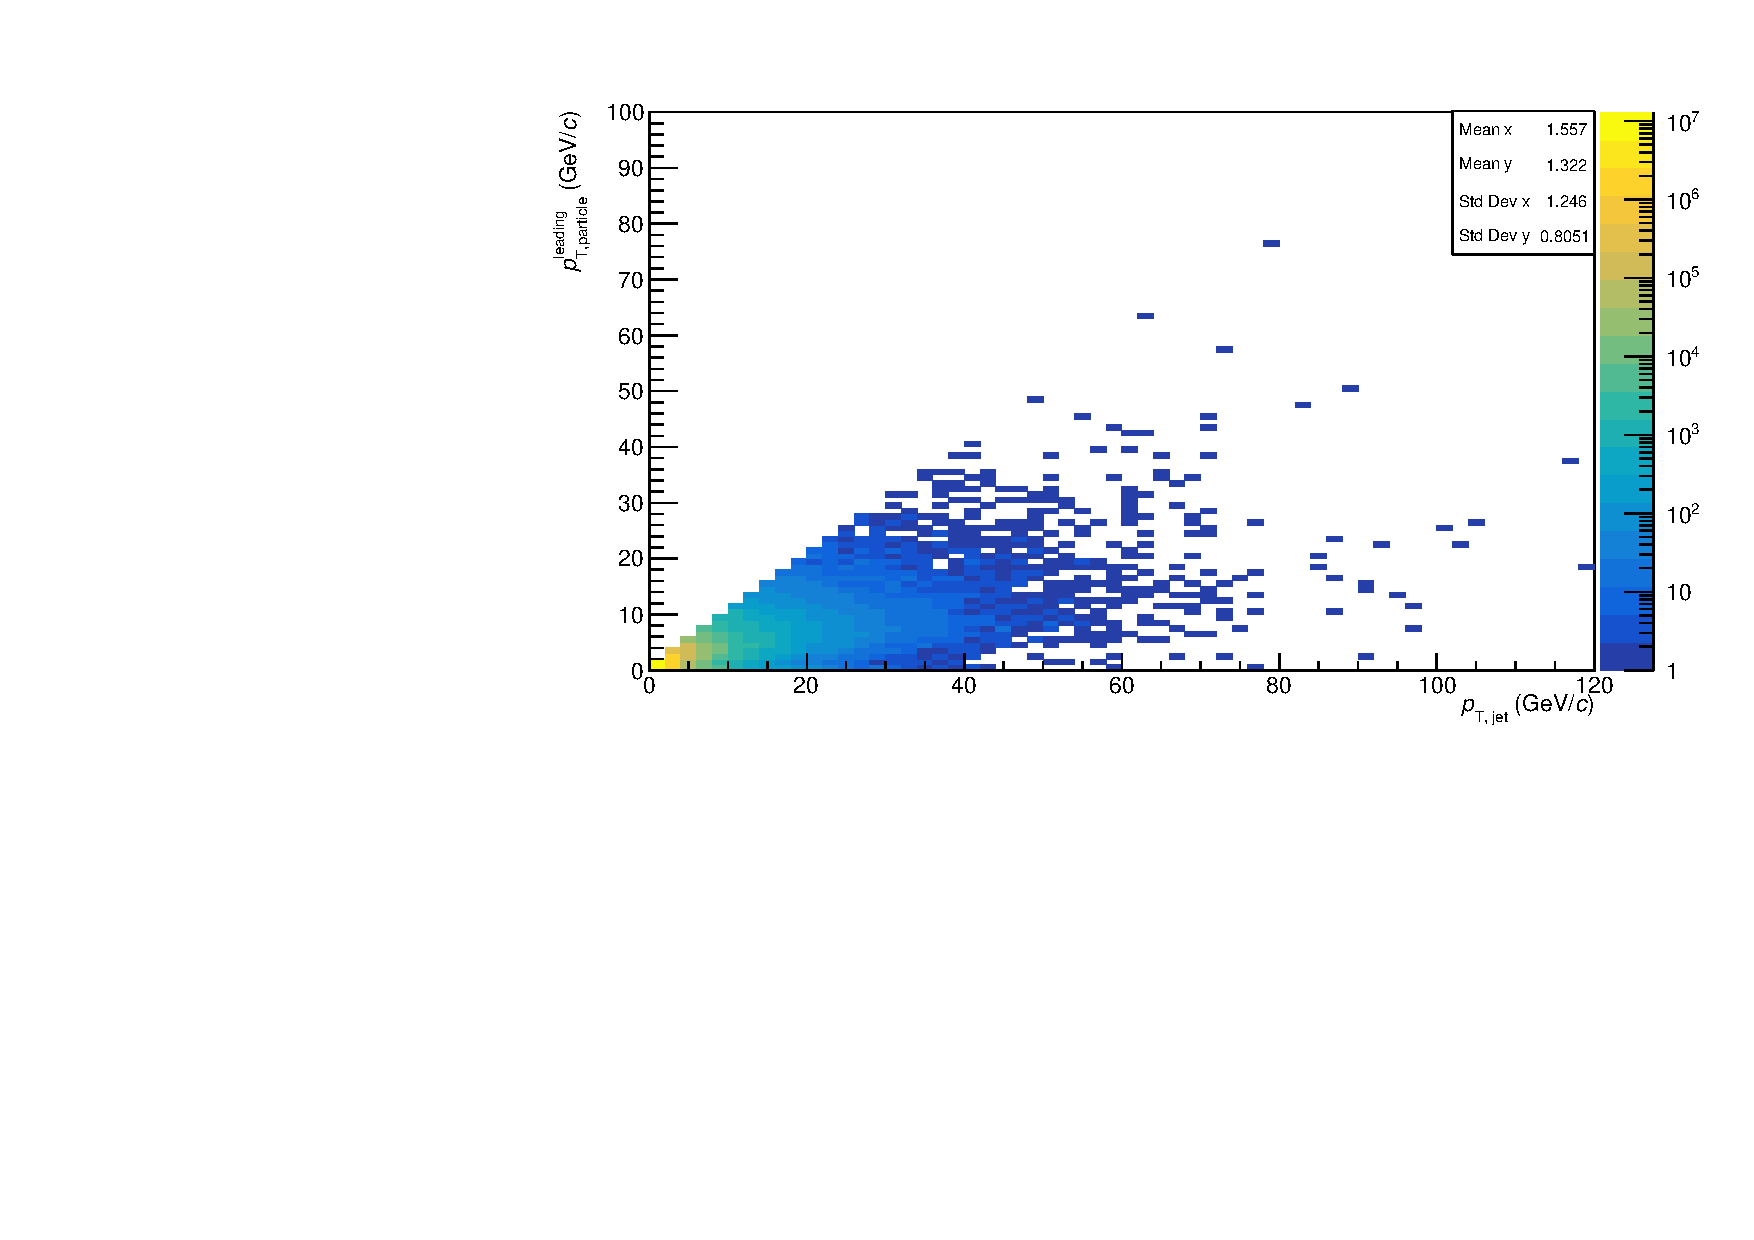
\includegraphics[width=8cm]{ptleadingR02}
\centering
\caption{R = 0.2 leading track $p_{T}$ per jet $p_{T}$.}
\label{fig:JetPt}
\end{figure}

\begin{figure}[h]
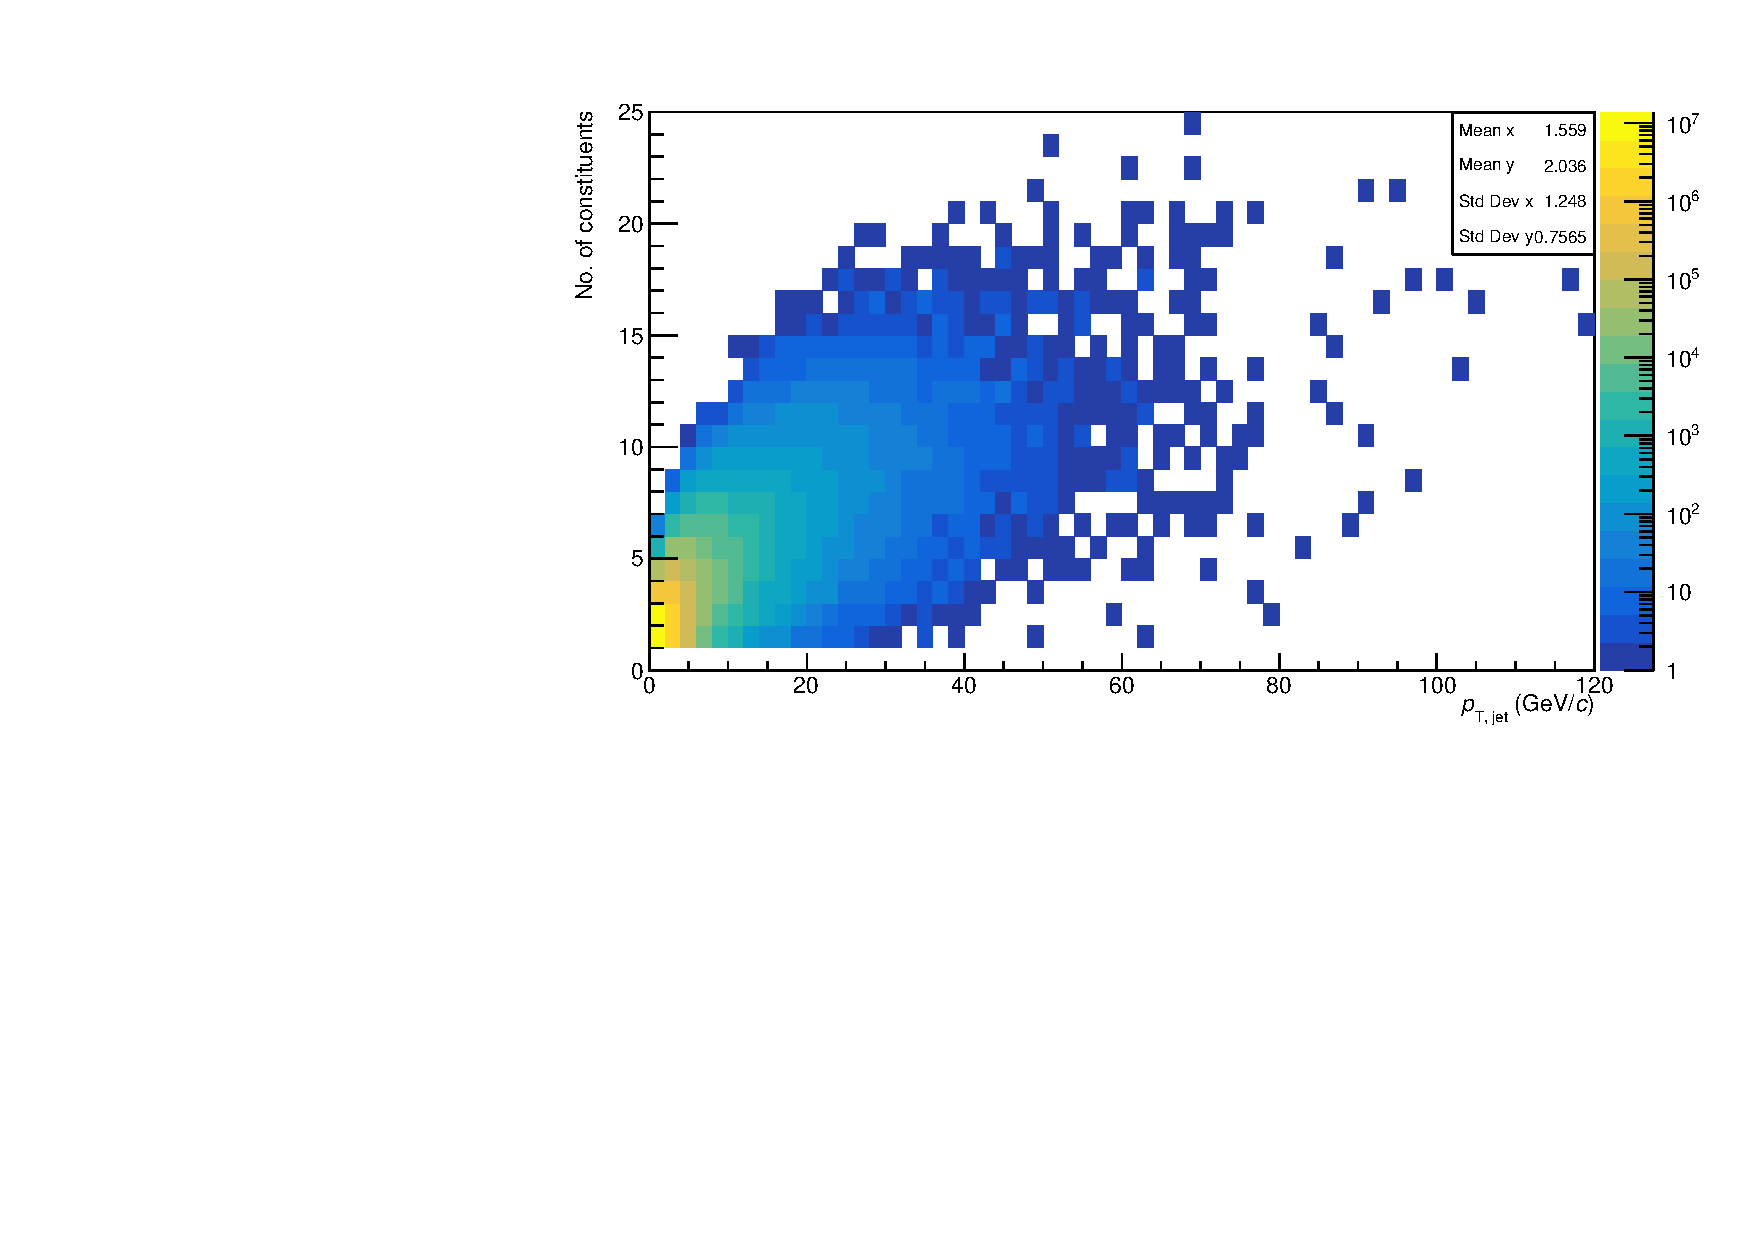
\includegraphics[width=8cm]{JetnumcconstR02}
\centering
\caption{R = 0.2 number of constituents in a jet per jet $p_{T}$.}
\label{fig:JetConst}
\end{figure}



\noindent
\subsection{$z_{leading}$ cut}

The fragmentation function for the leading track in a jet,

\begin{equation}
z_{leading} = \frac{ p_{leading, proj} }{ p_{jet} },
\label{eq:zleading}
\end{equation}

\noindent
may be artificially high due to misidentifiying secondary decay particles as primary vertex tracks and assigning them a much larger $p_{T}$.  Additionally, fake clusters, such as exotics, may skew the jet $p_{T}$ to apperantly large values and thus make $z_{leading}$ infinitesimal.  

\begin{figure}[h]
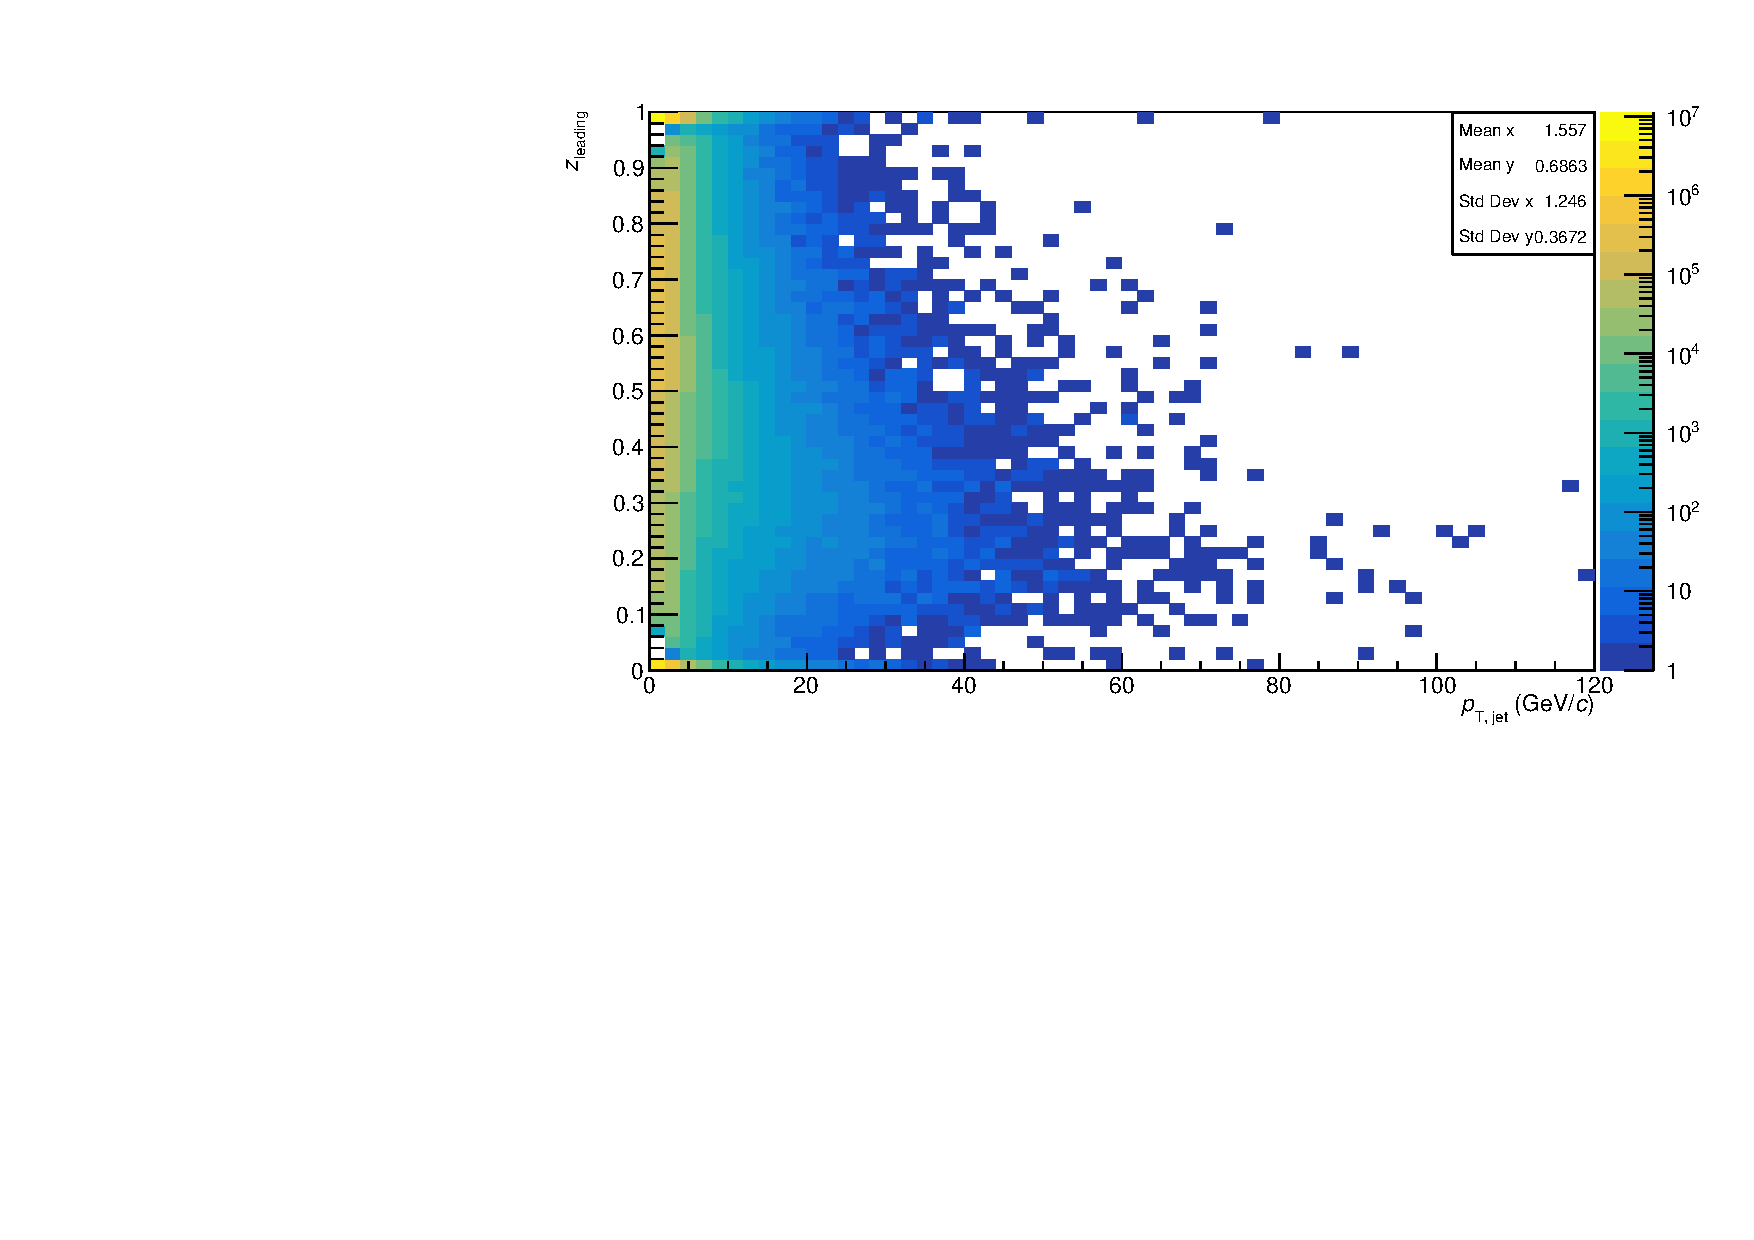
\includegraphics[width=10cm]{JetzR02}
\centering
\caption{R = 0.2 $z_{leading}$ from the Min Bias data sample.}
\label{fig:Jetz}
\end{figure}

\noindent
Figure \ref{fig:Jetz} shows the projection of the hadronic 3-momentum onto the jet axis.  We observer an excess of jets, especially at low jet $p_{T}$, of z values close to 1 or zero.  To help remove these biased jets a cut on $ z_{leading} \geq 0.03$ and $z_{leading} \leq 0.97$ is imposed.  It should also be noted that due to QCD hadronization $z_{leading} \sim 1$ corresponds to a singular particle jet which is highly rare.  Inbetween .03 and .97 we see the $z_{leading}$ is continuous and uniform as expected.  

\subsection{Jet Area Cut}

A jet area of, $A_{jet}$, cut was imposed on accepted jets.

\begin{equation}
A_{jet} \geq 0.6 \pi R_{jet}^{2}
\label{eq:AreaJet}
\end{equation}

The area is estimated in FastJet using `ghost' particles.  As jet reconstrution is being performed these fake particles with infinitesimal $p_{T}$ are placed randomly through the event.  The number of ghost particles captured in a jet is proportional to the jet area, thus the precision of the jet area is sensative to the reconstruction of soft particles.  Figure \ref{fig:jetrej} shows the rejection reason for a jet with the dominate reasoning due to the area cut and this distribution skewed towards loa-$p{T}$ jets.

\subsection{NEF cut}
The Neutral Energy Fraction (NEF) is the total jet energy carried by the neutral components of the jet, i.e. EMCal clusters.  Figure \ref{fig:JetNEF} shows the NEF for R = 0.2 jets from the Min Bias sample.

\begin{figure}[h]
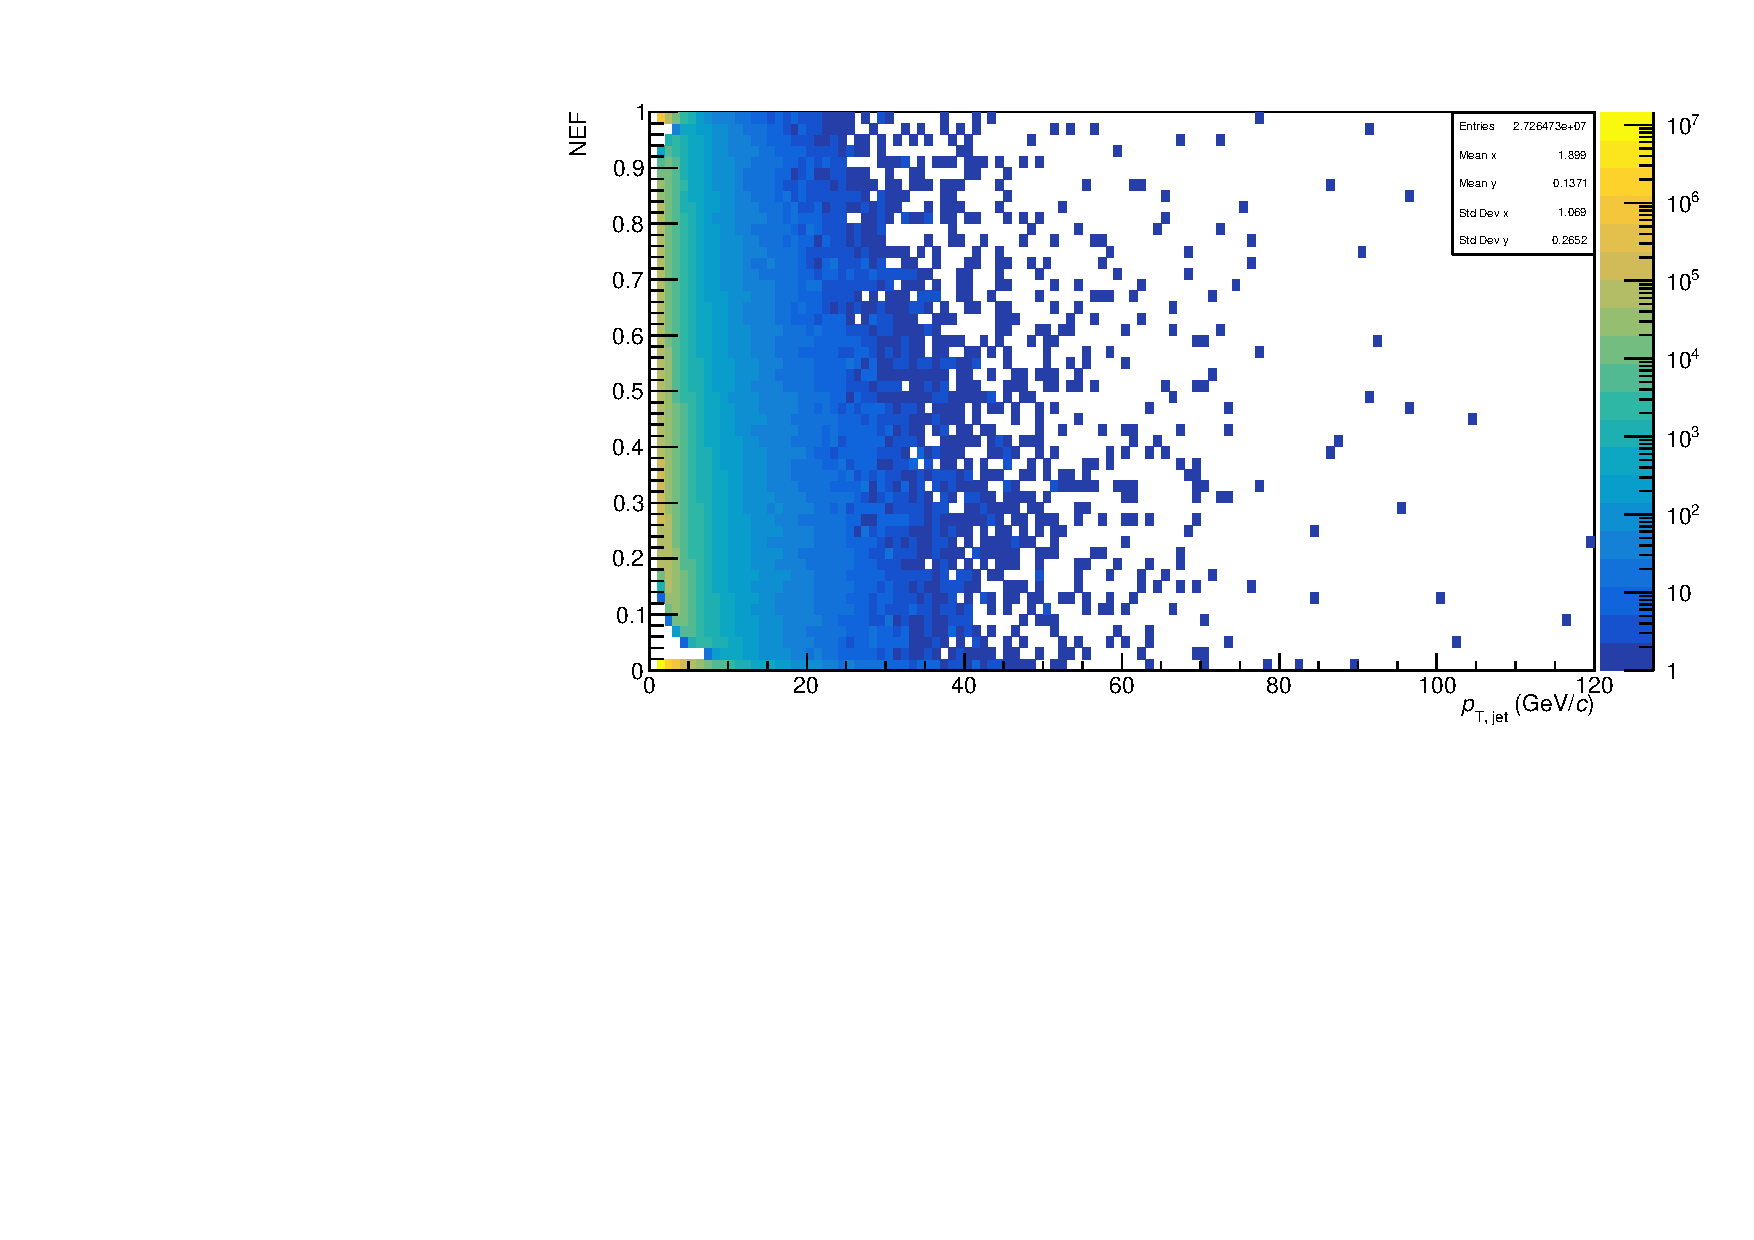
\includegraphics[width=10cm]{NEFR02}
\centering
\caption{R = 0.2 NEF per jet $P_{T}$.}
\label{fig:JetNEF}
\end{figure}
\noindent
We observe an excess in jets at low-$p_{T}$ with NEF values around zero or one, similar to what was seen with the $z_{leading}$ distribution.  The cause for these excesses were explored in this analysis but no hard source was identified and no cut to the NEF was used.

The jets the passed all of the selection criteria and cuts make up the signal jets that are reported in the cross section and spectra.  These criteria were implemented for the R = 0.3 and R = 0.4 along with the EMCal triggered data.




\section{EMCal Triggered Data}

In addition with the minimum bias data collected, the EMCal was used during the 8 TeV run in order to provided an enhanced data set that is preferential to hard processes.   The Level-1 trigger\cite{Bourrion:2010js} in the EMCal has a associated trigger, $\epsilon$, of 

\begin{equation}
	\epsilon = \frac{N^{Triggered}_{events}}{N^{MinBias}_{events}} \times \frac{d^{2} N_{Triggered}^{jet}}{d\eta \, dp_{T}} \Bigg/  \frac{d^{2} N_{MinBias}^{jet}}{d\eta \, dp_{T}} 
\label{eq:xsecdef}
\end{equation}

\subsection{Acceptance Correction}
Jet spectra, cross sections, and ratios of cross sections are reported over the full azimuth angle and psuedorapidity acceptance.  However, due to jets being constrained to the EMCal, a geometric factor is used to correct for the limited acceptance of the detector.  This thesis uses a maximum jet radius of 0.5 to help study the effects of wide angle radiation on jet fragmentation.  Heavy-ion use smaller jet radii, typically of 0.2, to help negate the high multiplicity background.  Due to these geometric corrections the centroid of a jet is constrained to,

\begin{equation}
|\eta_{jet}| \leq 0.7 - R, \; 1.4 + R \leq \phi_{jet} \leq 3.14 -R.
\label{eq:jetconstration}
\end{equation}

\begin{equation}
A(p_{T}) = \frac{(1.4 - 2R) \times (1.745 - 2R)}{2 \pi}.
\label{eq:acceptance}
\end{equation}

For jets between R = 0.1 through R = 0.5 the following jet acceptance corrections are used.

\begin{table}[hb]
\label{tab:AcceptanceFactor}
\begin{center}
\begin{tabular}[b]{|c|c|c|}
	\hline
	Jet R & $A(p_{T})$ \\ \hline
	0.1 & 0.296 \\ \hline
	0.2 & 0.214\\ \hline
	0.3 & 0.146\\ \hline
	0.4 & 0.091\\ \hline
	0.5 & 0.048\\ \hline
\end{tabular}
\end{center}
\caption{EMCal jet acceptance for radii 0.1 - 0.5.}
\end{table}








\section{Unfolding}

The reconstructed jet $p_{T}$ has a number of detector effects `folded' into the measurement.  These effects included such things as:

\begin{itemize}
\item Tracking inefficiencies from the TPC and ITS.
\item Missing jet energy components from long-lived particles, such as the $K^{0}_{L}$ and neutron, that are cut by the EMCal timing requirement.
\item TPC track $p_{T}$ and EMCal cluster energy resolutions.
\item Hadronic corrections to the EMCal cluster spectrum.
\item Material loss in the detectors.
\end{itemize}

\noindent
Unfolding is the method by which these detector effects are removed from the raw inclusive jet spectra and a `true' jet spectra may be obtained and compared with theoretical calculations or other experimental results.  In order to unfold a jet spectra it is necessary to generate a response matrix that simulates the described effects above, after the response matrix is generated a number of statistical approaches including, Bayesian, Singular Value Decomposition (SVD), or Bin-by-Bin, may be applied to unfold the raw jet spectra.  In order to generate the response matrix we embed a Pythia generated event into a GEANT3 simulation of the ALICE detector.  Due to the fact that the performance and efficiency of the ALICE detector may change between the data taking periods each simulation is `anchored' to a given LHC, these anchors contain all the hot and dead sectors for the subdetectors, along with their calibrated performance during that specified data taking.  Two Monte Carlo data sets were produced with the MB trigger for the full 8 TeV run, the first was a Pythia generator using the Monesh-2013 tune and the second was a MB tune of the PHOjet Monte Carlo package.  Both data sets were explored for this thesis and it was decided that the final corrected spectra would be obtained via unfolding with the Pythia MC data set.  The magnitude of any one of the effects unfolding is supposed to account for is not expected to be very large, but combined may be significant, thus unfolding is an important step in this analysis.

\subsection{Response Matrix}
Given a truth-level particle jet $p_{T}$ we wish to reconstruct that jet's $p_{T}$ at the detector-level.  The particle-level pythia jets are constructed from the primary particles generated via Pythia while excluding any daughter decay particles in order to avoid double counting.  In addition the tracking efficiency in Pythia is known to deviate from nature.  This is due to Pythia under predicting the production of strange quarks.  
Constructing the response matrix in this case is calculated on a jet-by-jet basis.  The particle-level jet centroid ($\phi_{part}$,$\eta_{part}$)is matched to the detector-level jet via a constrain on the displaced distance between the two jet centroids in ($\phi$,$\eta$).  This distance was constrained to: $\Delta  R = \sqrt{(\phi_{part} - \phi_{det})^{2} + (\eta_{part} - \eta_{det})^{2}} \leq 0.25 \; $.  Once a jet is matched at the detector level to a jet generated from the particle level the response matrix is incremented by jet $p_{T}$ at both the detector and Monte Carlo levels.  The response matrix is generated with a fine binning with a width of 1 GeV per bin. 

\begin{figure*}[t!]
$\begin{array}{rl}
    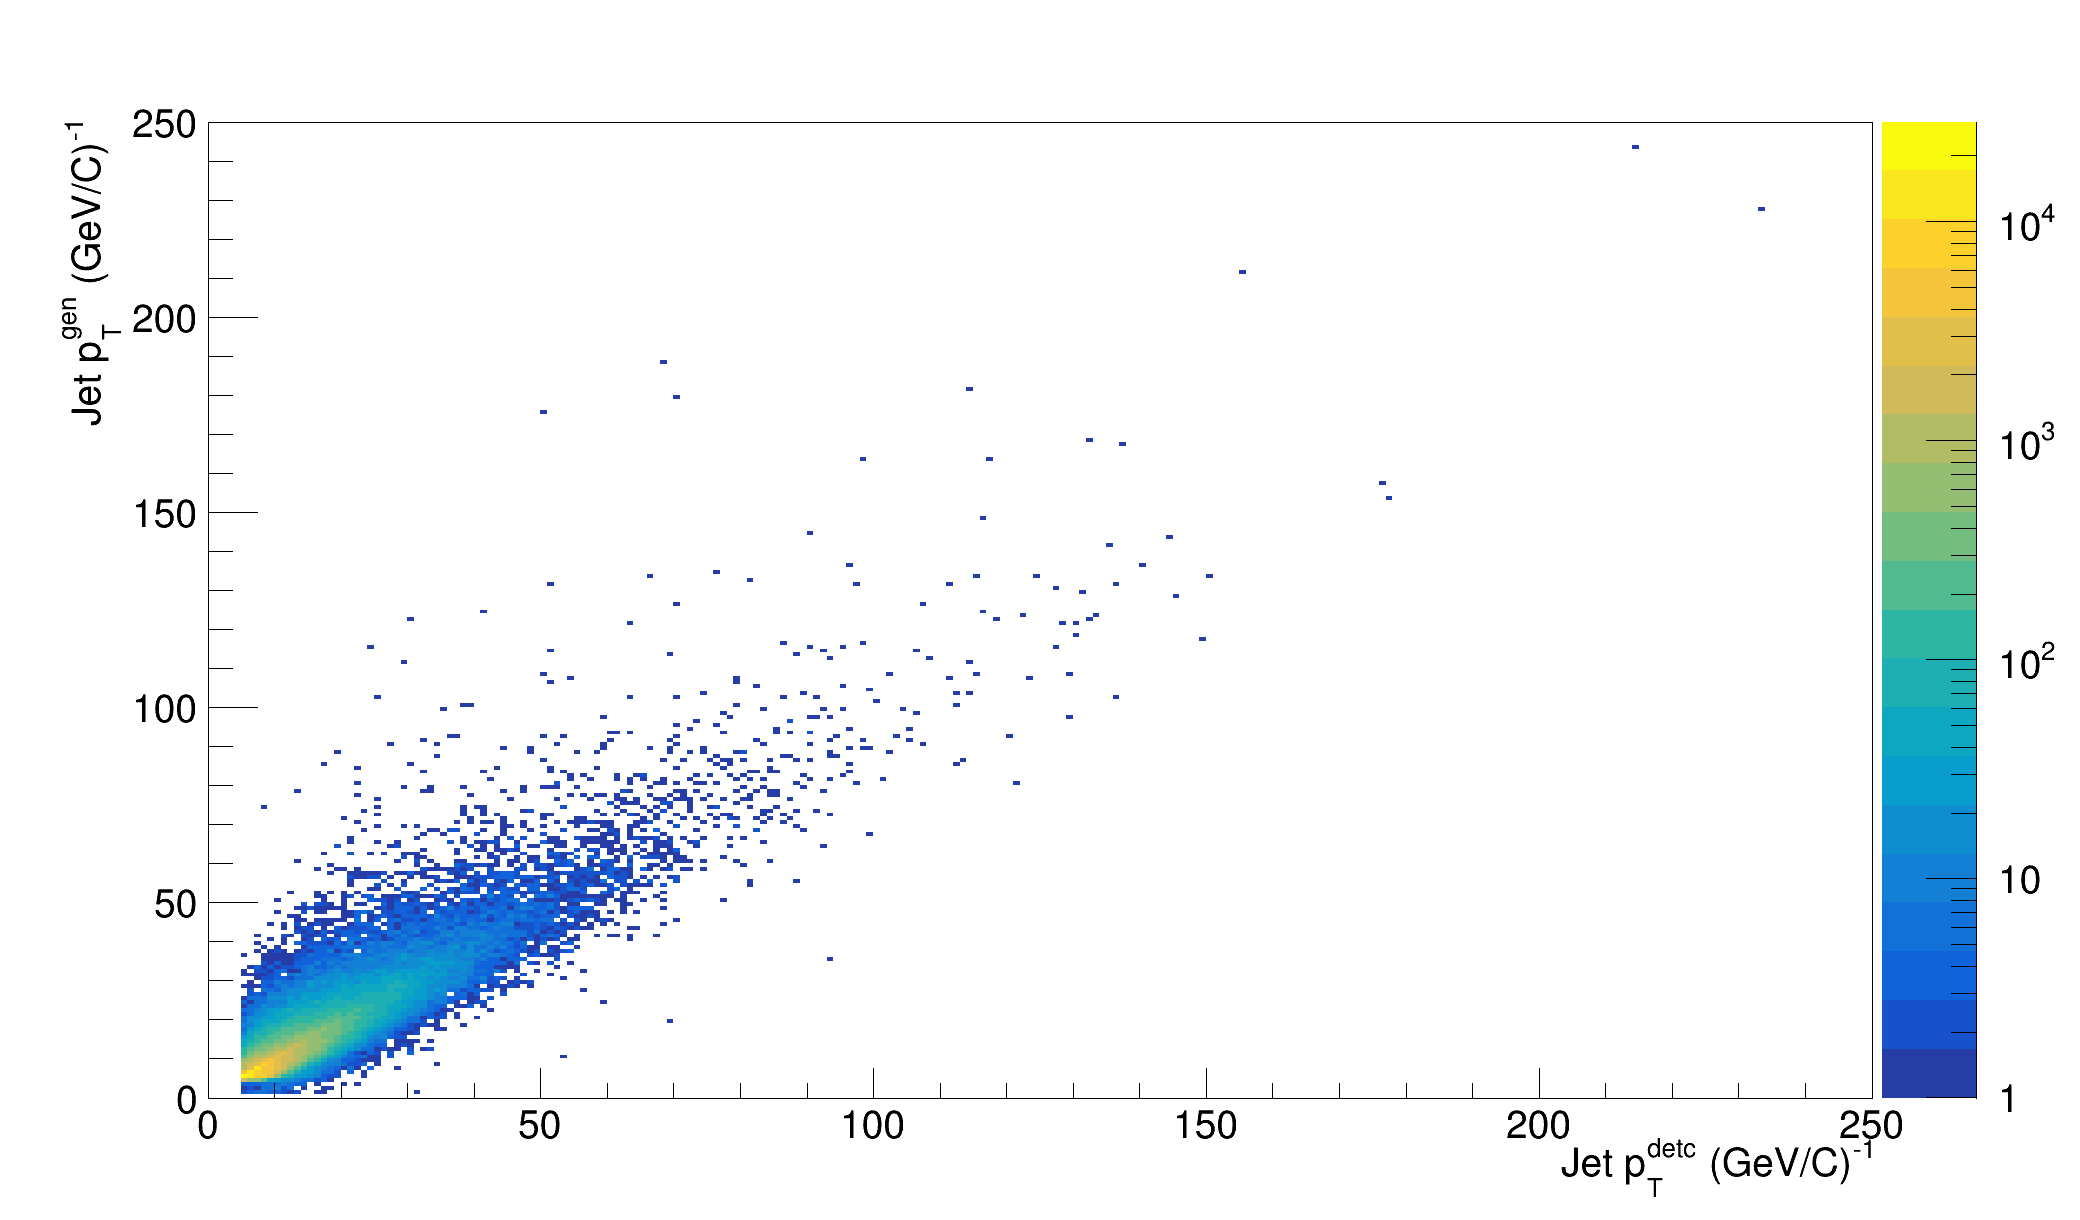
\includegraphics[width=0.5\textwidth]{responseR02} &
    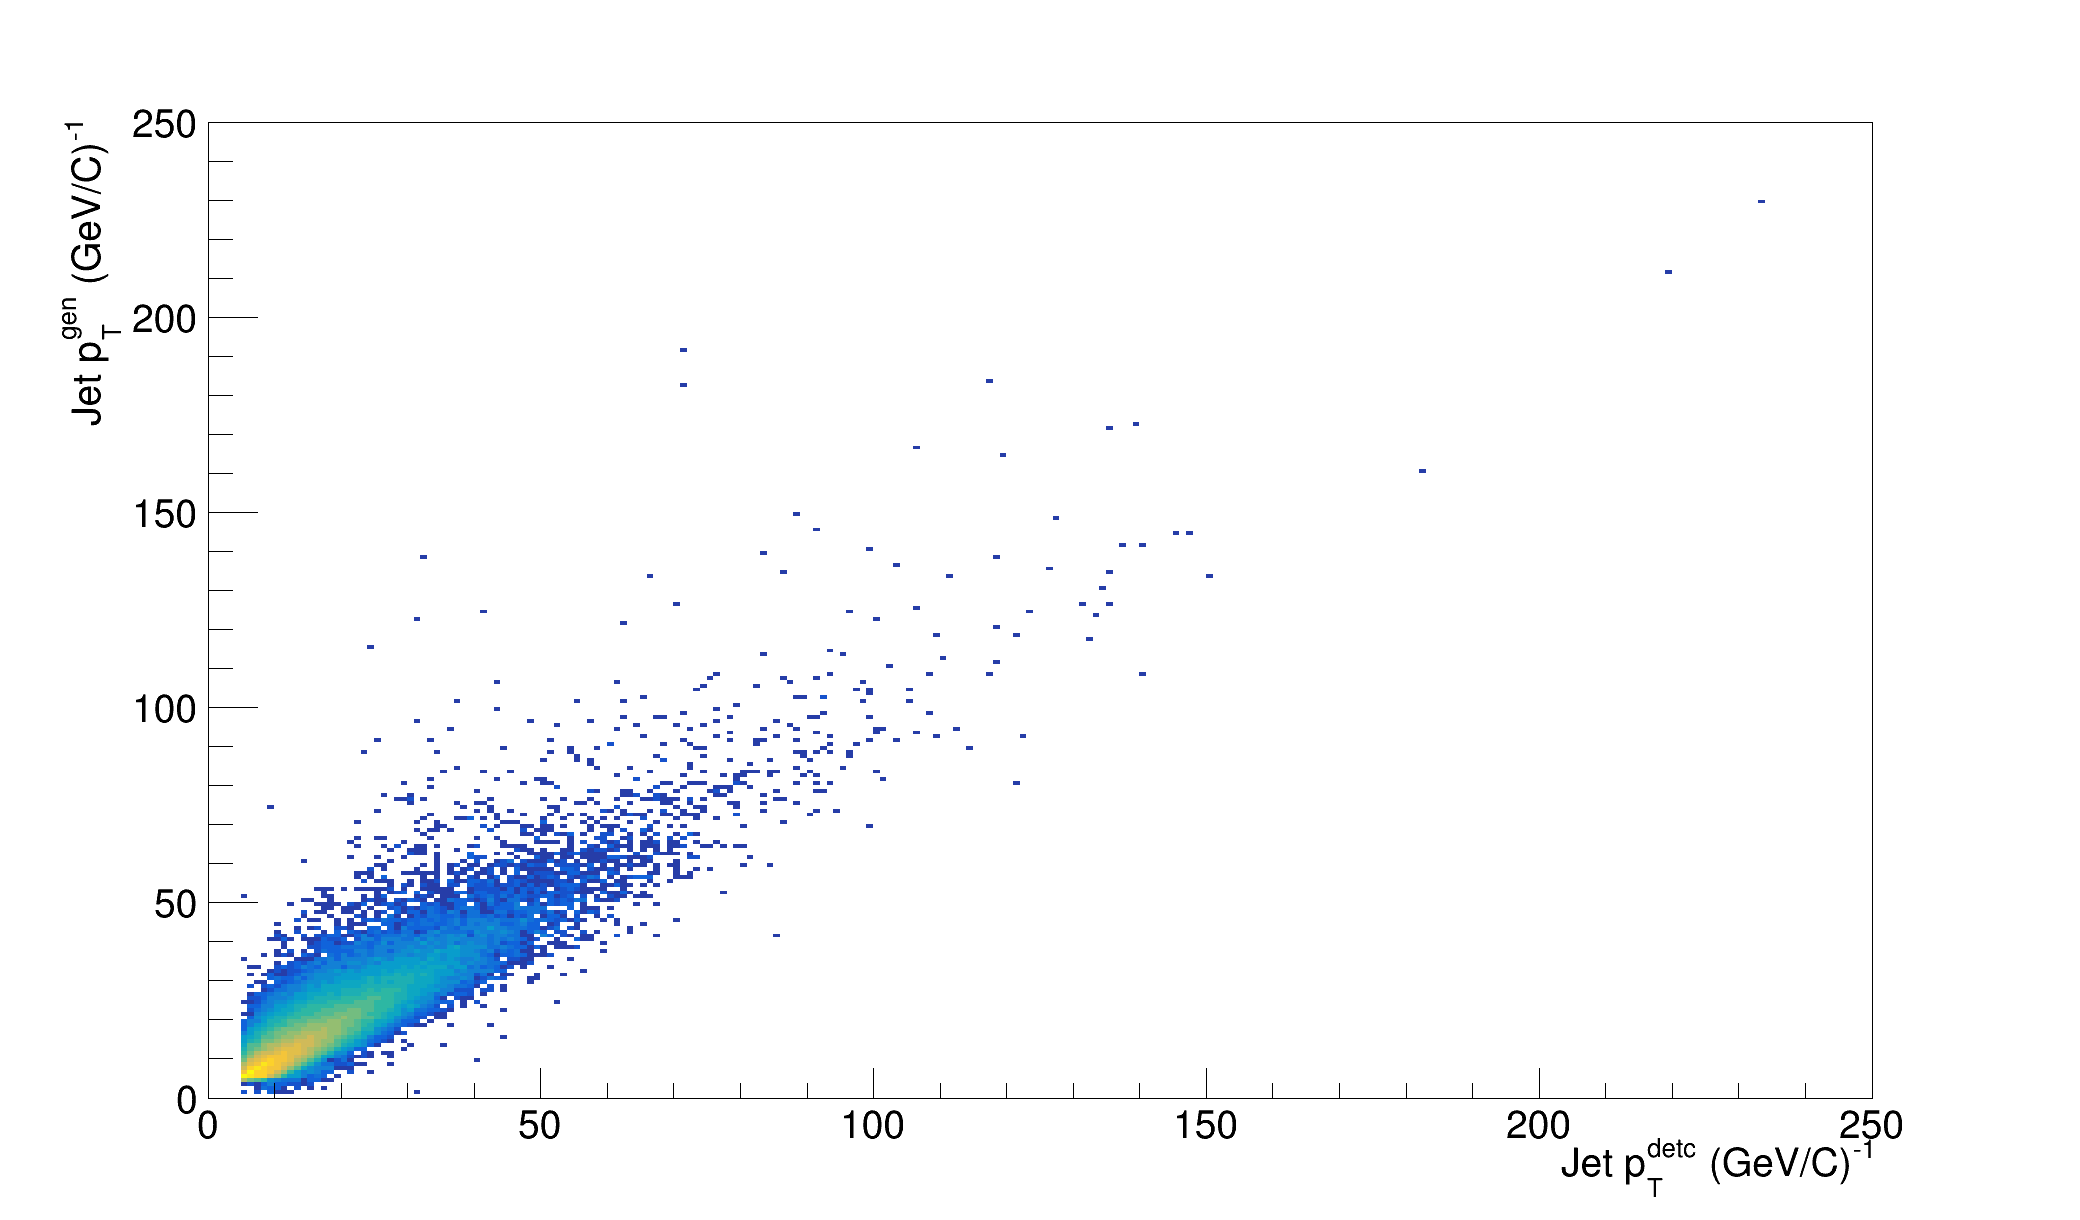
\includegraphics[width=0.5\textwidth]{responseR03}\\
    \multicolumn{2}{c}{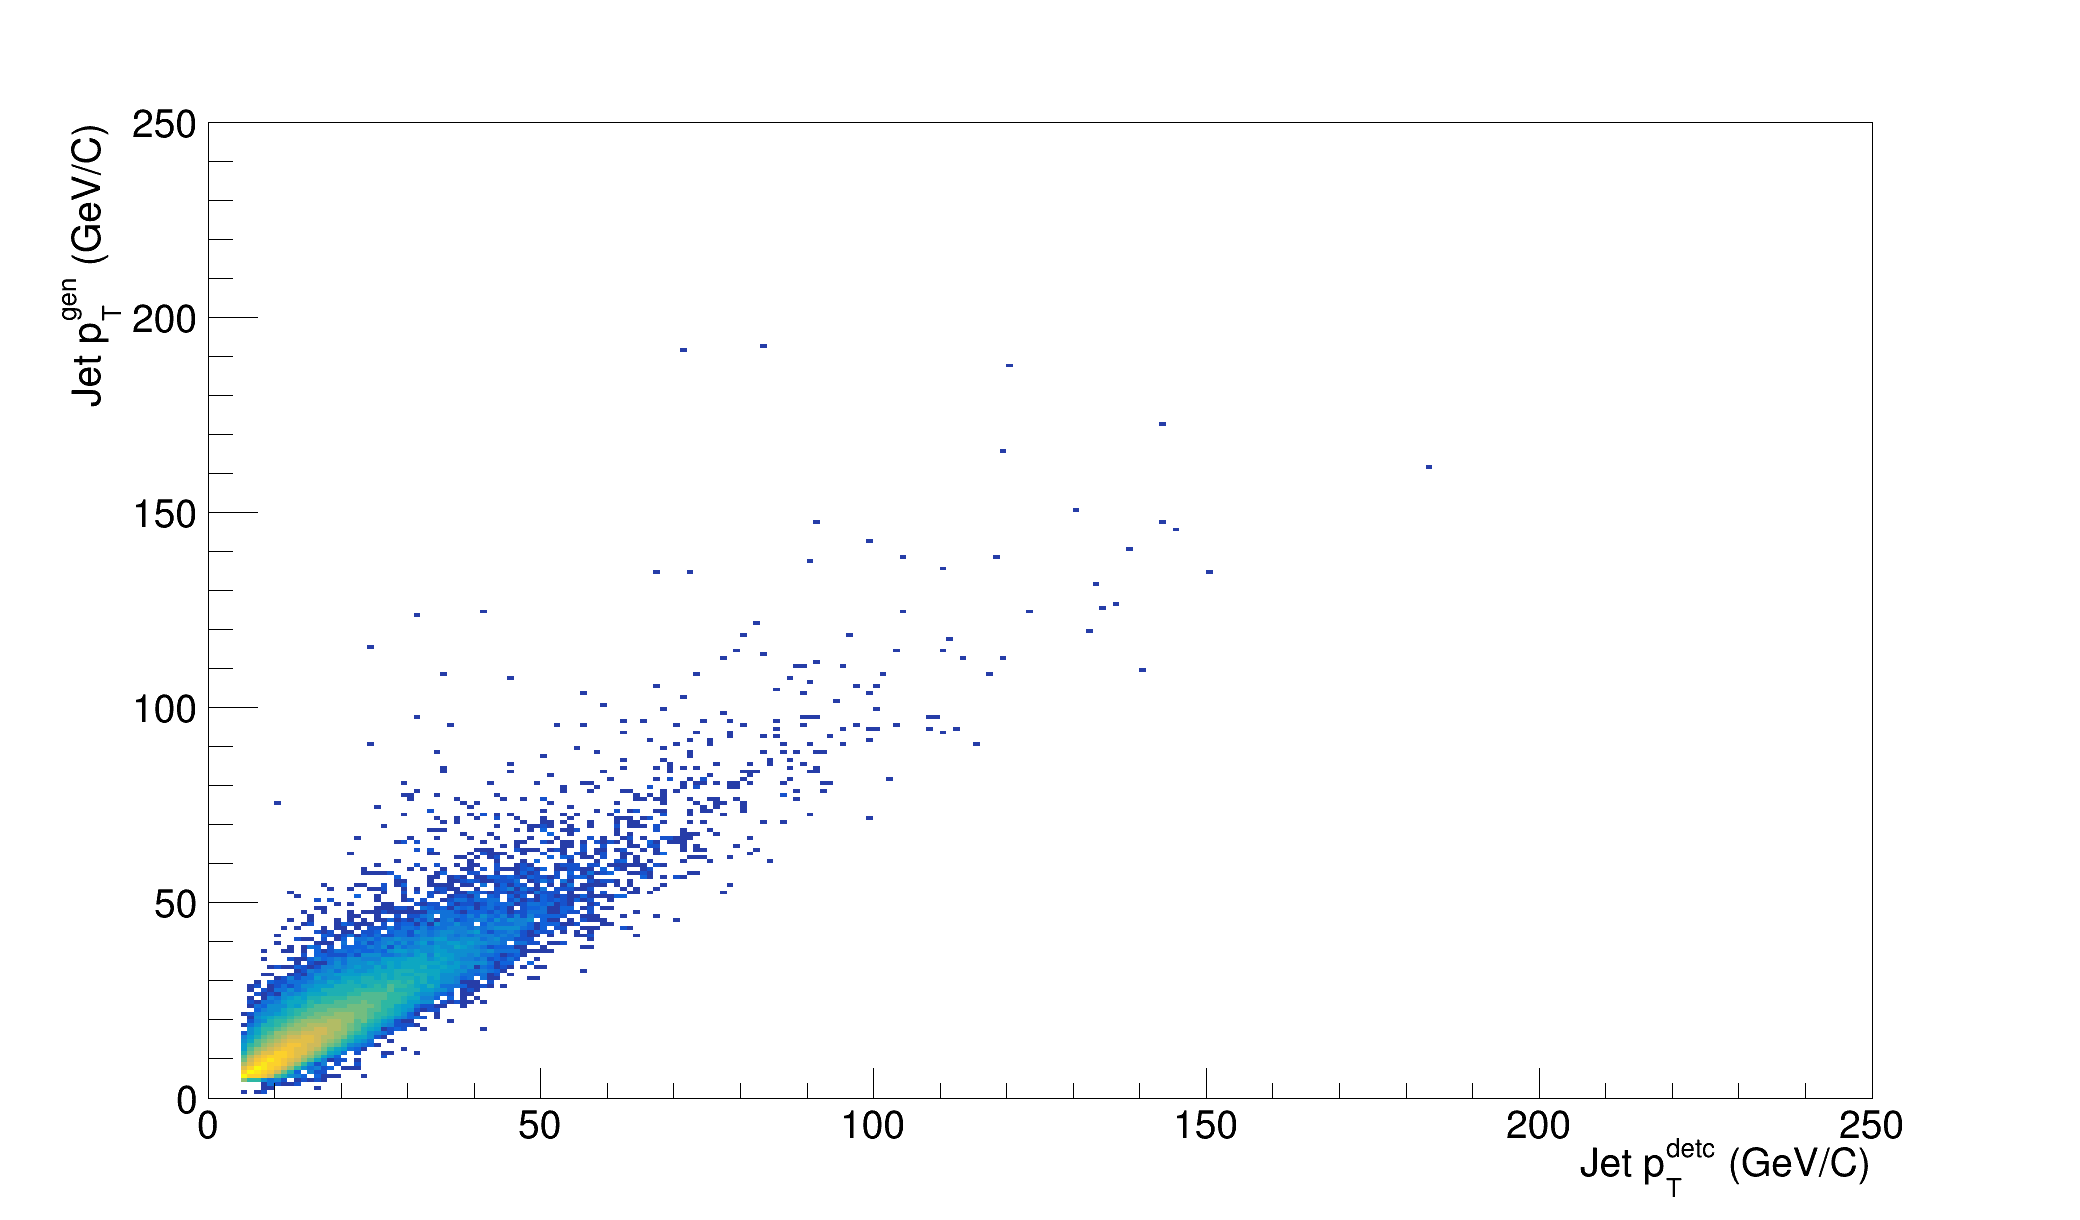
\includegraphics[width=0.5\textwidth]{responseR04}}
\end{array}$
\caption[Response Matrices for R = 0.2, R=0.3, and R = 0.4 jets.]{\label{fig:response}Response Matrices for R = 0.2, R=0.3, and R = 0.4 jets.}
\end{figure*}

Figure \ref{fig:response} shows the response matrices for the R = 0.2 (top left), R = 0.3 (top right), and R = 0.4 (bottom) jets generated with the prescribed manner.  The response matrices display a linear relationship below 50 GeV on both axis and above ~ 100 GeV the matrices are statistics starved.  This is primarily due to the Monte Carlo Pythia and PhoJet data sets generated for the 8 TeV pp run did not model the high-$p_{T}$ triggers associated with the EMCal.  The particle jet finders configured for the response matrices allowed for jet finding down to a 100 MeV jet candidate at the particle level with no constraints on the minimum particle momentum or energy for a constituent.  The detector level jet finders were configured in the same manner as the jet finders configured for the raw jet spectra measurement.  

\subsection{Corrections to Particle Level}

Unfolding was performed using the \verb+RooUnfold+\cite{Adye:2011gm} software package.  Corrections are applied using the bin-by-bin\cite{Cowan:2002in} algorithm. 

\begin{equation}
C_{MC} \big( p_{T}^{low} : p_{T}^{high} \big) =  \frac{  \int^{p_{T}^{high}}_{p_{T}^{low}} dp_{T} \; \frac{dF^{uncorr}_{meas}}{dp_{T}} \times \frac{d^{2}N^{particle}_{MC}/d\eta \, dp_{T}}{d^{2}N^{detector}_{MC}/d\eta \, dp_{T}}  } { \int^{p_{T}^{high}}_{p_{T}^{low}} dp_{T} \; \frac{dF^{uncorr}_{meas}}{dp_{T}} }
\label{eq:binbybin}
\end{equation}

\noindent
where $d^{2}N^{particle}_{MC}/dp_{T} \, d\eta$ is the PYTHIA level inclusive jet spectra, $d^{2}N^{detector}_{MC}/dp_{T} \, d\eta$ is the GEANT 3 level inclusive jet spectra, $dF^{uncorr}_{meas} / dp_{T}$ is a weight function which minimizes the dependence on the two simulation spectra shapes, finally $p_{T}^{low}$ and $p_{T}^{low}$ are the lower and upper bin limits.  Due to the limited statistics derived from the Monte Carlos available the unfolding procedure was stable only in aunfolding the truth level jet spectra for the range: $p_{T,jet} \epsilon \;$ [10 GeV, 120 GeV] for both the raw Min Bias and Emcal triggered data sets.  Due to the  the final truth value for the jet spectra will be reported in this range.



\subsection{Unfolded MB Spectra}

\begin{figure}[h]
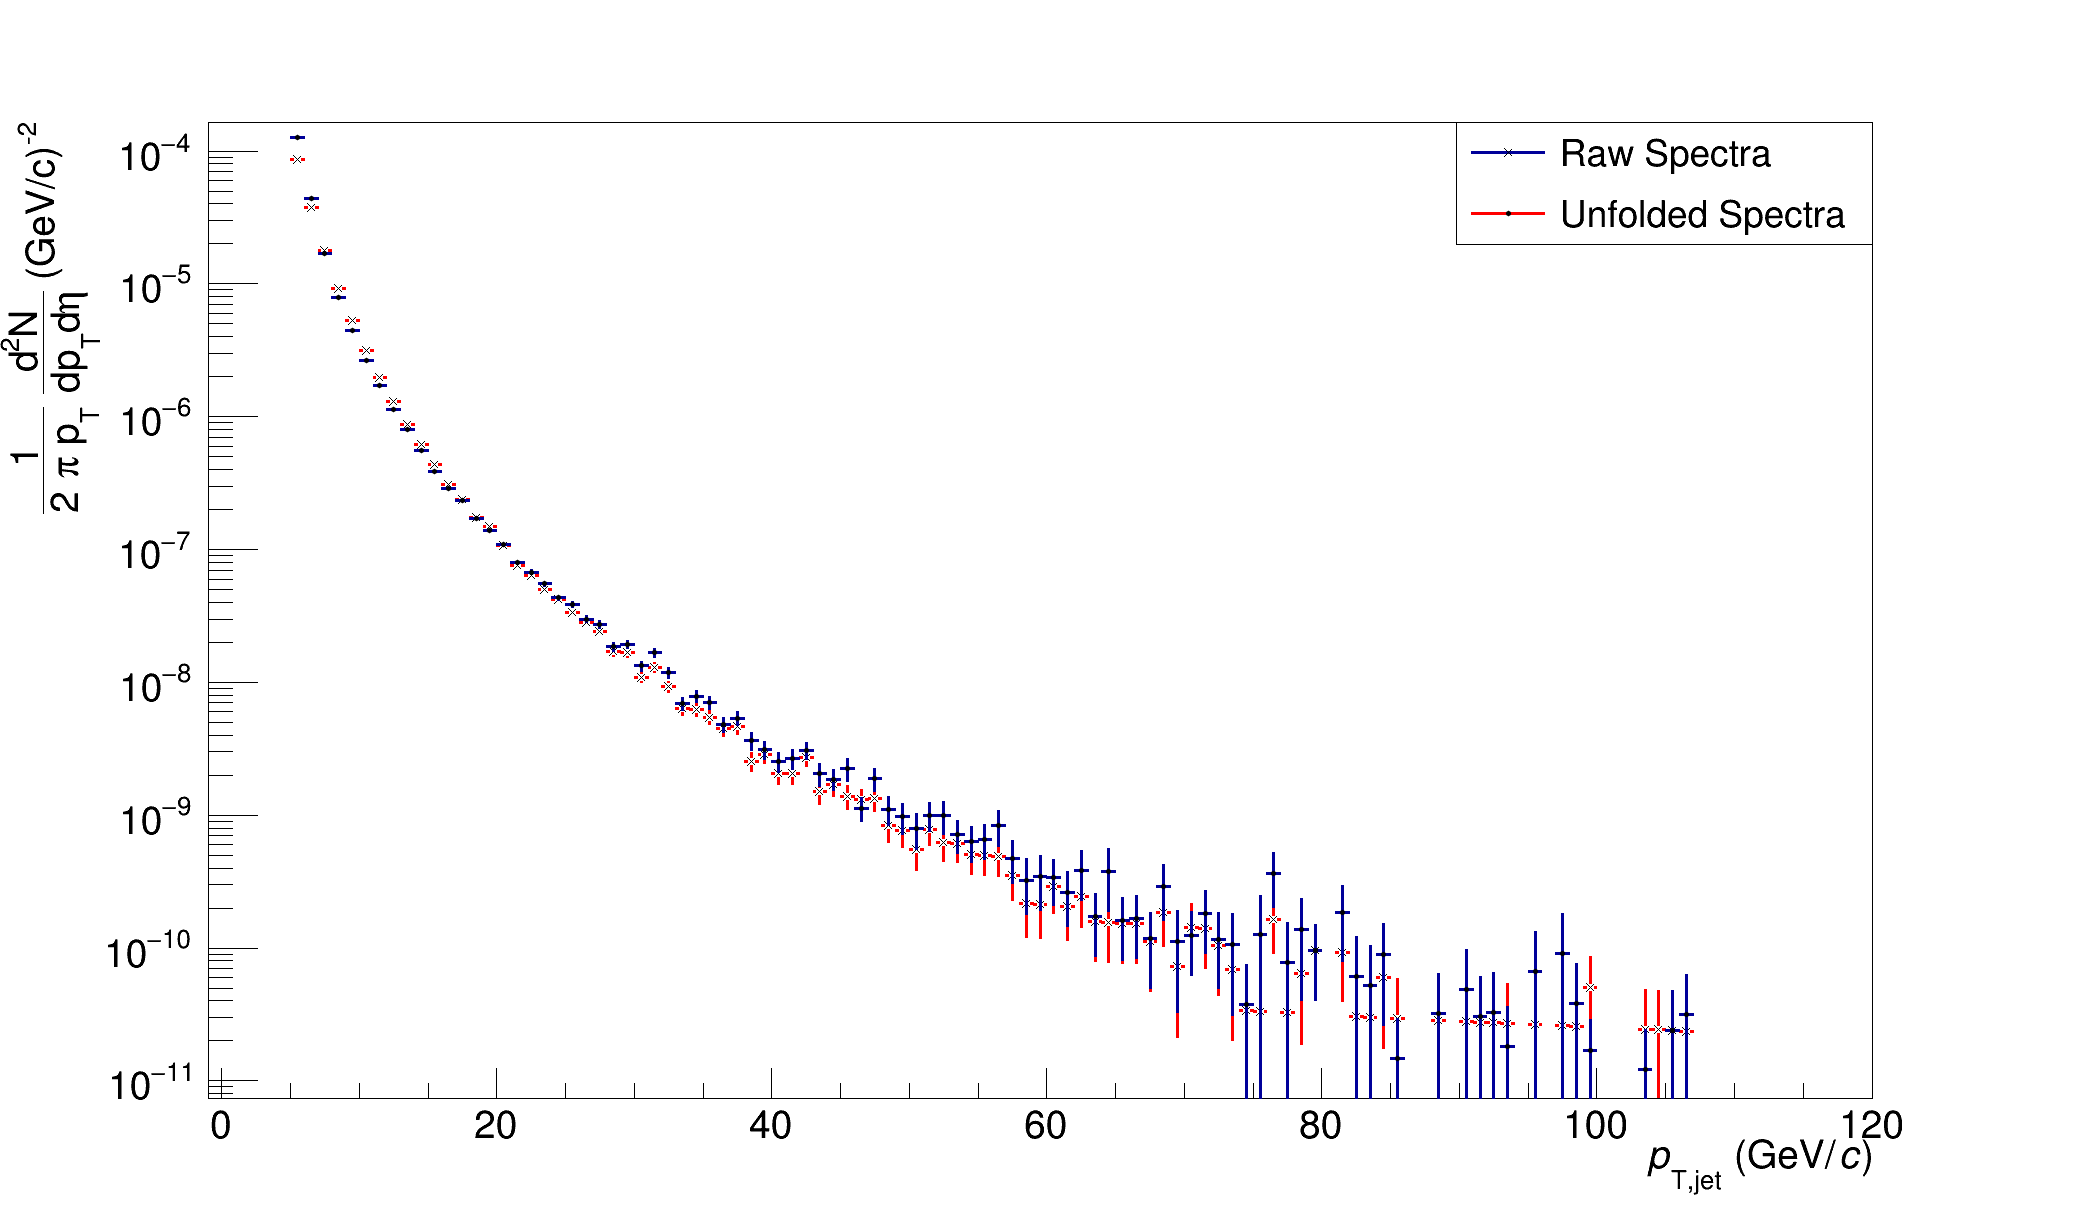
\includegraphics[width=13cm]{RawandUnfoldedSpectraMBR03}
\centering
\caption{Unfolded jet spectra with fine binning for R = 0.3}
\label{fig:Unfoldfine}
\end{figure}

Figure \ref{fig:Unfoldfine} shows an example of the output from the bin-by-bin unfodling with the fine binning for R = 0.3 jets.  It should be noted that at low-$p_{T}$ it was observed that unfolding increased the yield of the spectra while at high-$p_{T} \geq \,$ 40 GeV the yield was decreased for all jet radii in this analysis.  This is most likely due to the lack of statistics in the response matrix.  Once the bin-by-bin unfolding has been performed for the fine binned spectra the output along with the bin-by-bin correction factors ar rebinned using a variable binning between 10 GeV and 120 GeV.

\begin{figure}[h]
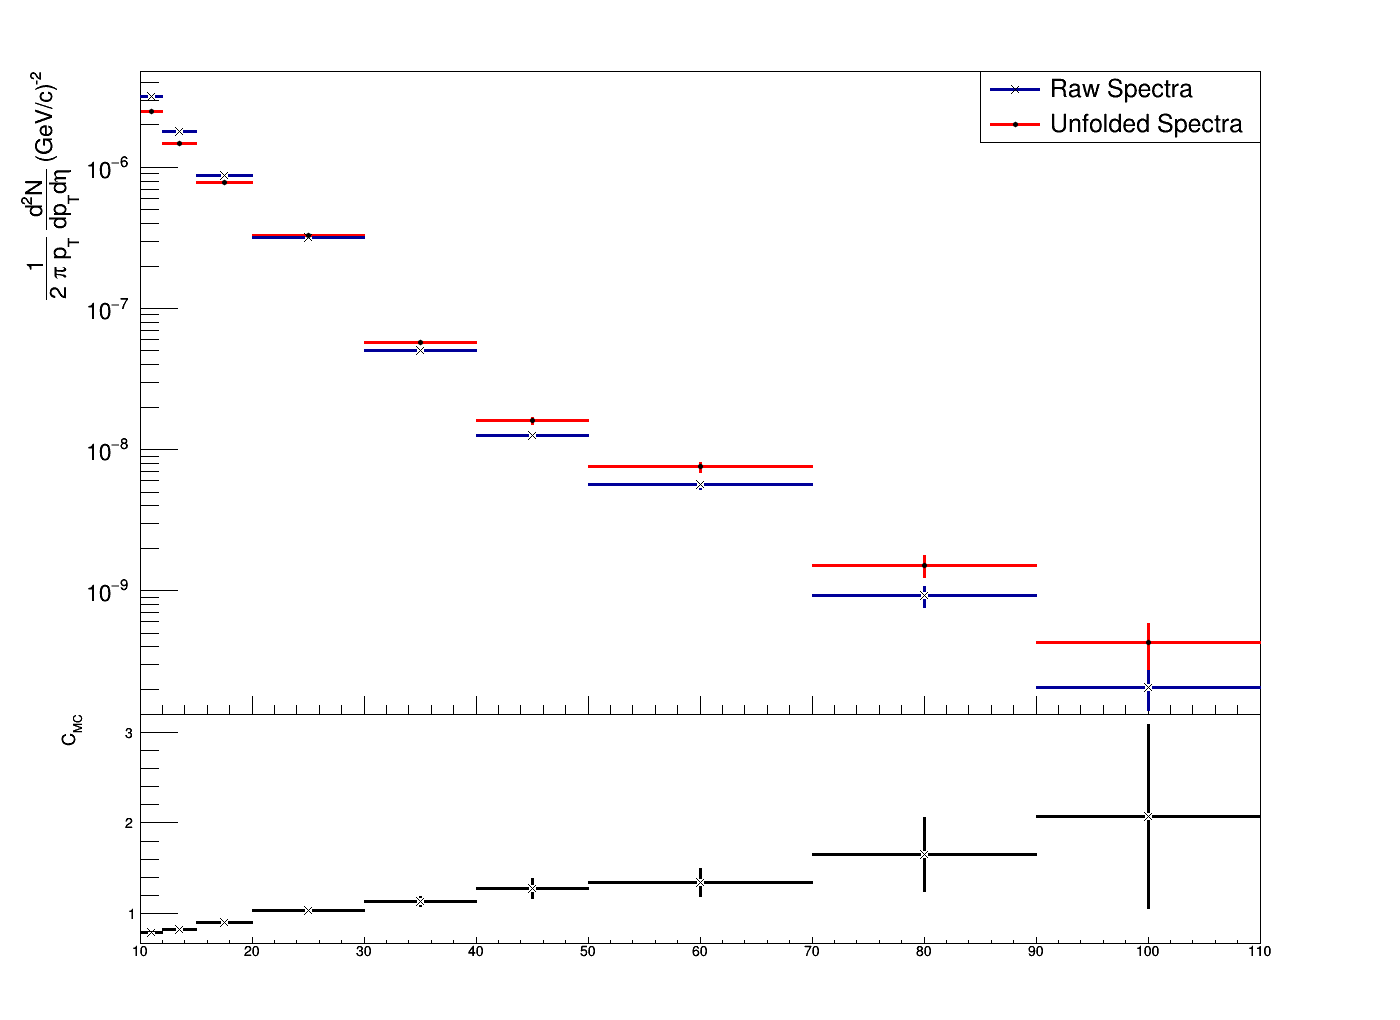
\includegraphics[width=10cm]{UnfoldedR02MinBias}
\centering
\caption{Unfolded Min Bias R = 0.2 jet spectra with corrections factors using a variable binning.}
\label{fig:UnfoldvarR02}
\end{figure}

\begin{figure}[h]
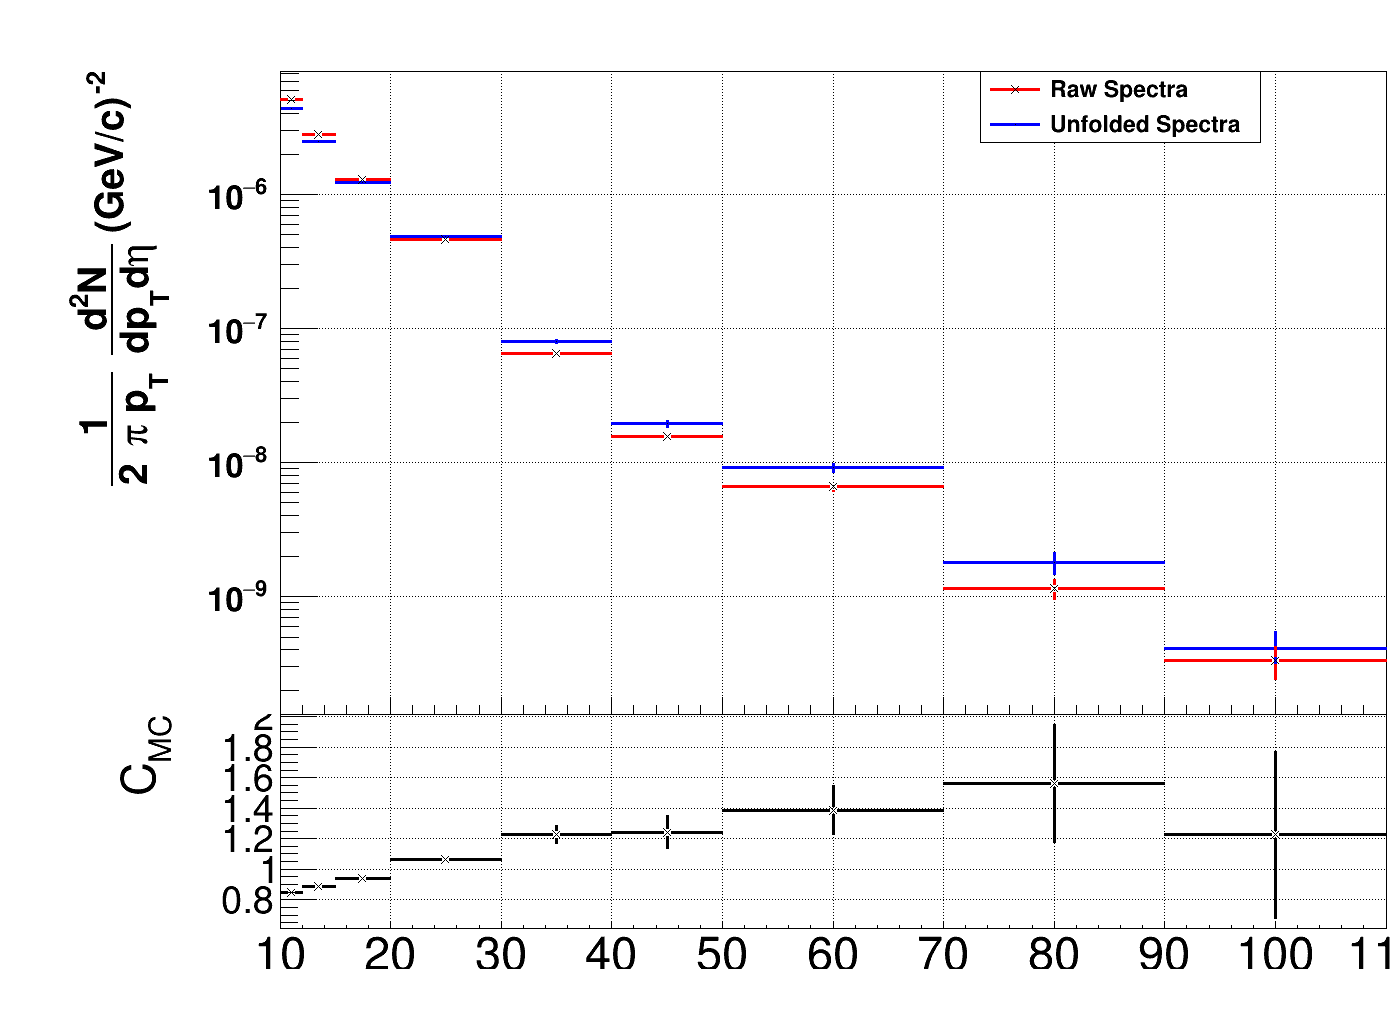
\includegraphics[width=10cm]{UnfoldedR03MinBias}
\centering
\caption{Unfolded Min Bias R = 0.3 jet spectra with corrections factors using a variable binning.}
\label{fig:UnfoldvarR03}
\end{figure}

\begin{figure}[h]
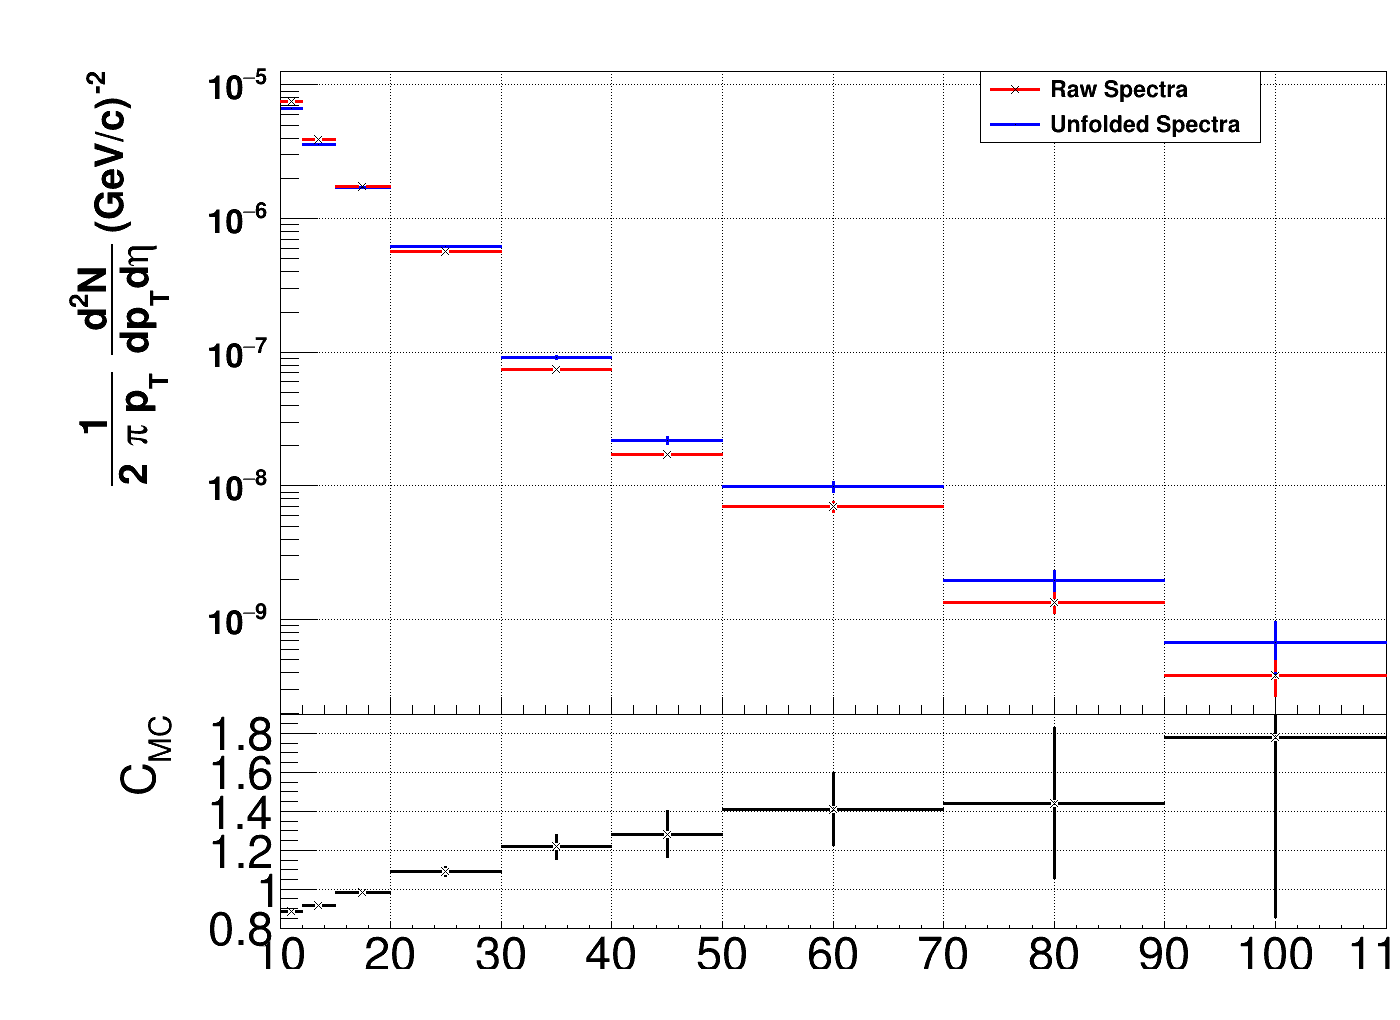
\includegraphics[width=10cm]{UnfoldedR04MinBias}
\centering
\caption{Unfolded Min Bias R = 0.4 jet spectra with corrections factors using a variable binning.}
\label{fig:UnfoldvarR04}
\end{figure}


\subsection{Unfolded EMCal Triggered Spectra}
The unfolding procedure is repeated again for the EMCal triggered jet spectra.  The response matrix from the Min Bias sample is used for the bin-by-bin unfolding and performed using a fine binning.  The detector level and particle level jets are configured in the same manner as above and the output from the unfolded triggered specta are reported after rebinning to a variable size over the same kinematic range as the Min Bias sample.

\begin{figure}[h]
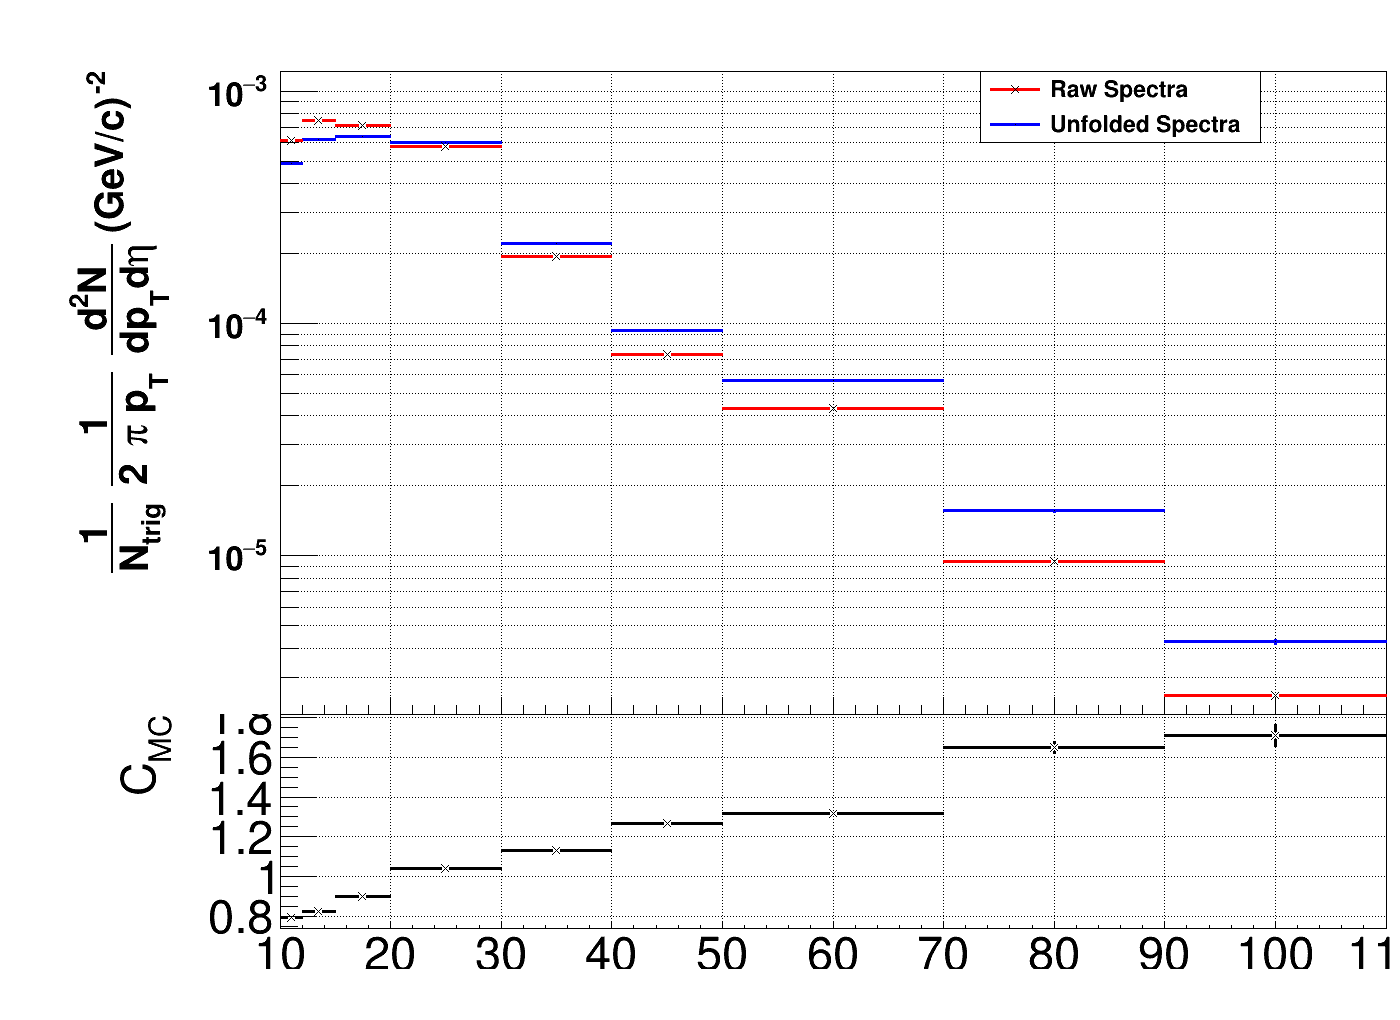
\includegraphics[width=10cm]{UnfoldedR02EGAtrigger}
\centering
\caption{Unfolded EMCal triggered R = 0.2 jet spectra with corrections factors using a variable binning.}
\label{fig:UnfoldvarR02EGA}
\end{figure}

\begin{figure}[h]
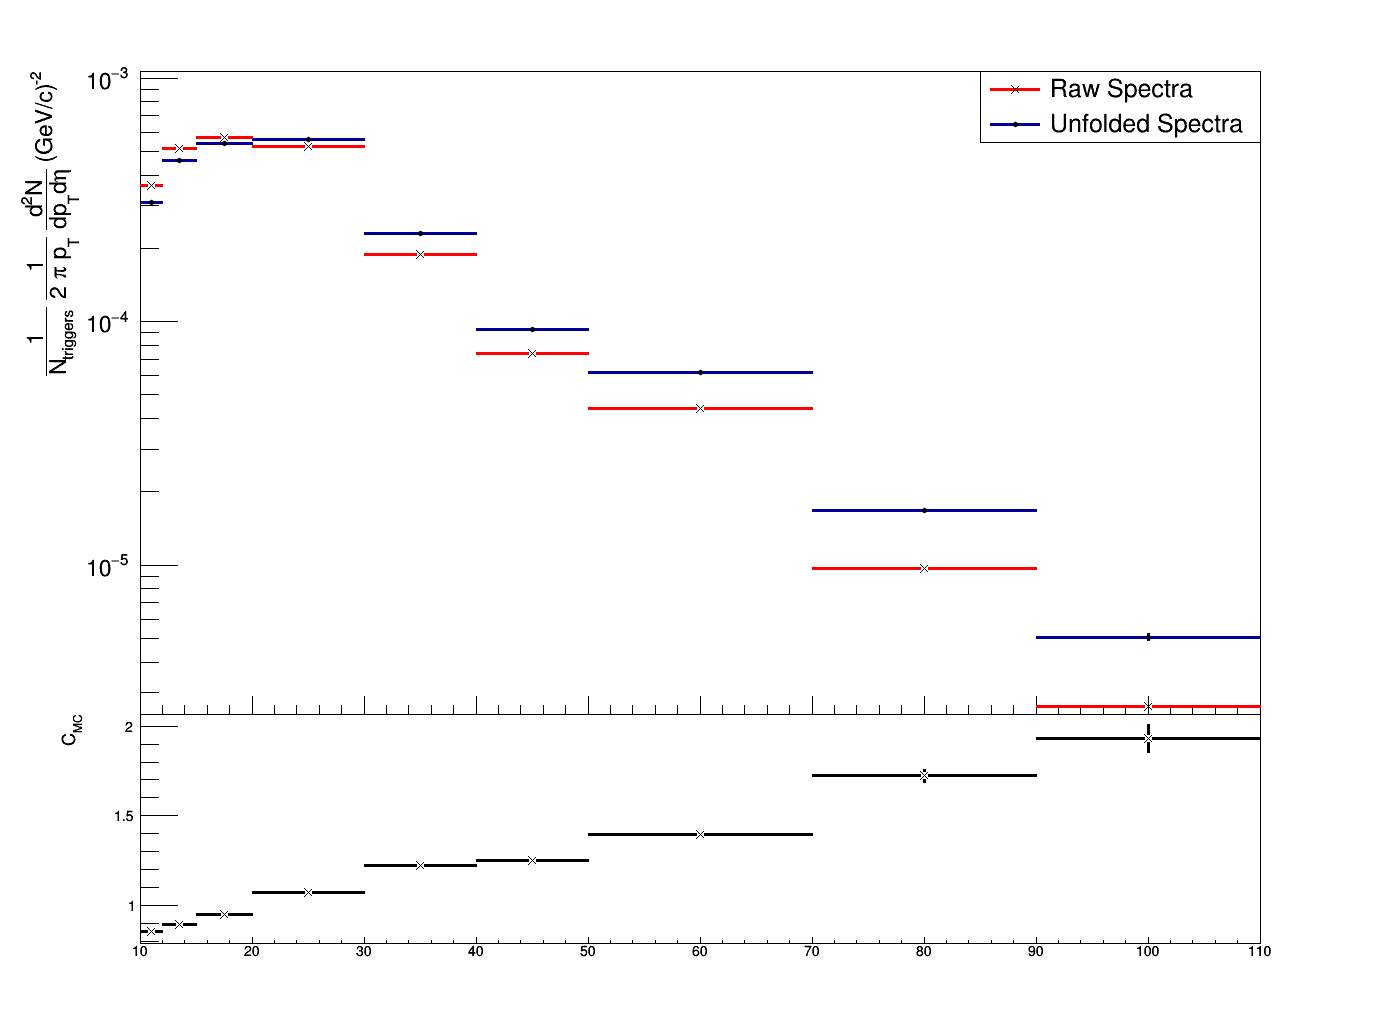
\includegraphics[width=10cm]{UnfoldedR03EGAtrigger}
\centering
\caption{Unfolded EMCal triggered R = 0.3 jet spectra with corrections factors using a variable binning.}
\label{fig:UnfoldvarR03EGA}
\end{figure}

\begin{figure}[h]
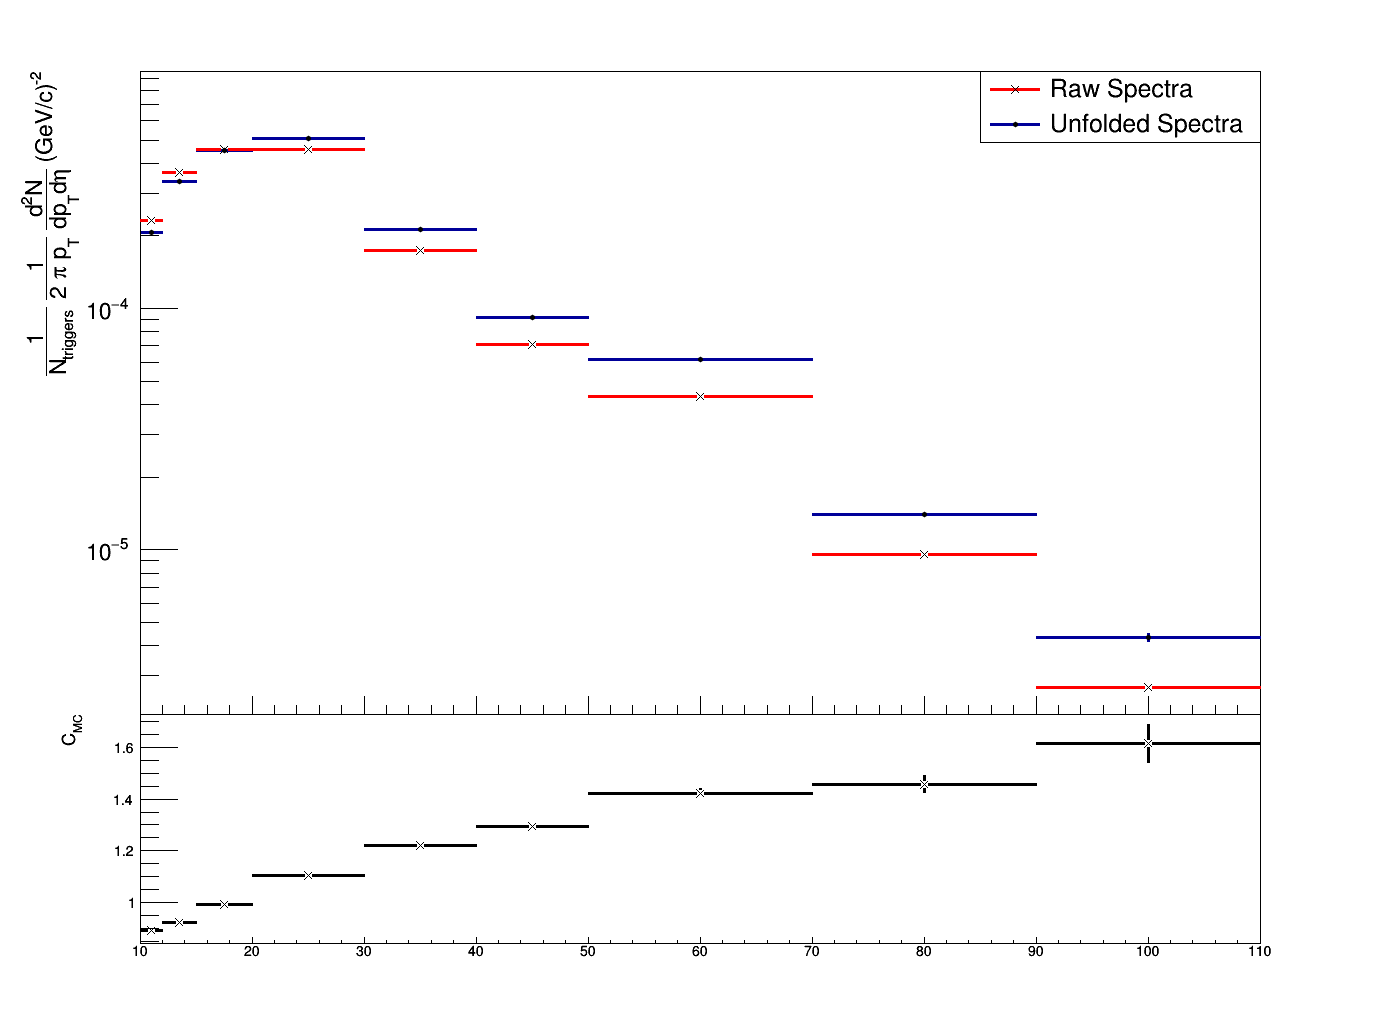
\includegraphics[width=10cm]{UnfoldedR04EGAtrigger}
\centering
\caption{Unfolded EMCal triggered R = 0.4 jet spectra with corrections factors using a variable binning.}
\label{fig:UnfoldvarR04EGA}
\end{figure}

\noindent
Due to the limitations on the response matrix the bin-by-bin unfolding of the EMCal triggered data was only stable up to 120 GeV.  It should be noted that the hump in the EMCal jet spectra is due to the firing threshold of the trigger.  The unfolded Emcal jet spectra was used to estimate the ratio the the jet yields between the Min Bias and triggered data samples, from this point the trigger scaling was calculated.  Due to the lack of a trigger modeled with the 8 TeV Monte Carlo productions the inability to extend the kinematic range of the jet spectras beyond 120 GeV presents a missed oppurtunity in terms of the recorded data from the 8 TeV runs.  In order to address this issue a new Monte Carlo production will need to be requested from the ALICE collaboration.

\subsection{Jet Reconstruction and Matching Efficiency}
In order to quantify the inefficiencies due to unfolding along with inefficencies in the ALICE experiment in reconstructing jets we quantify the jet reconstruction efficiency, $\epsilon_{reco} (p_{T, jet})$, and the jet matching efficiency, $\epsilon_{match} (p_{T, jet})$.

\begin{equation}
 \epsilon_{reco} (p_{T, jet}) = \frac{N_{reco}(p_{T, jet}) }{N_{Truth} (p_{T, jet})}
\label{eq:jetrecoeff}
\end{equation}

\begin{equation}
 \epsilon_{match} (p_{T, jet}) = \frac{N_{match}(p_{T, jet}) }{N_{Truth}(p_{T, jet})}
\label{eq:jetmatchoeff}
\end{equation}

\noindent 
where $N_{reco} (p_{T, jet})$ is the reconstructed jet yield at the detector level per $p_{T}$ bin, $N_{match}(p_{T, jet})$ is the reconstructed jet at the detector level that was matched to a particle level jet per $p_{T}$ bin, and $N_{truth} (p_{T, jet})$ is the truth-level jet yield from the Pythia embedded event per $p_{T}$ bin.  These quantities 

\section{Systematic Uncertainties}

Systematic uncertainties arise due to our limited knowledge of the precise operating conditions and performance of the experiment and also due to any bias in our understanding of how to fundamental model the interactions.  They systematics may therefore be broken into two components: uncertainties to the jet energy scale (JES) which shifts the momentum spectra along the x-axis and uncertainties in the jet yield which shift the spectra along the y-axis.  The systematical and statistical uncertainties presented in this analysis will be presented as errors to the yield of the spectra.  Due to the fact that the $p_{T}$ distribution follows a power law function, $dN/dp_{T} \sim p_{T}^{-5}$ uncertainties in the JES are converted to yield uncertainties by dividing each one by 5.
Due to the low statistics at the highest $p_{T}$ bins in this analysis, uncertainties in this regime my have large statistical fluctuations.  Small ,systematic variations for the input of the jet spectra will have a dramatic effect over sparsely filled bins versus bins with a low granularity.  As such it may be necessary to extrapolate the systematic from a low $p_{T}$ bin to those at the highsest $p_{T}$ range.  The systematics were performed on both the MB and EMCal triggered data samples but no large variation was observed between the two, thus only the uncertainties from the MB sample are shown and are extrapolated to the triggered data.


\subsection{Systematic Uncertainty to Jet Energy Scale}

\subsubsection{Tracking Efficiency}
Corrections for the tracking efficiency were performed by randomly throwing out 5\% of the tracks from each event from the 8 TeV data samples and reperforming jet on the altered data.  All of the inputs for jet finding were maintained.


\begin{figure*}[t!]
$\begin{array}{rl}
    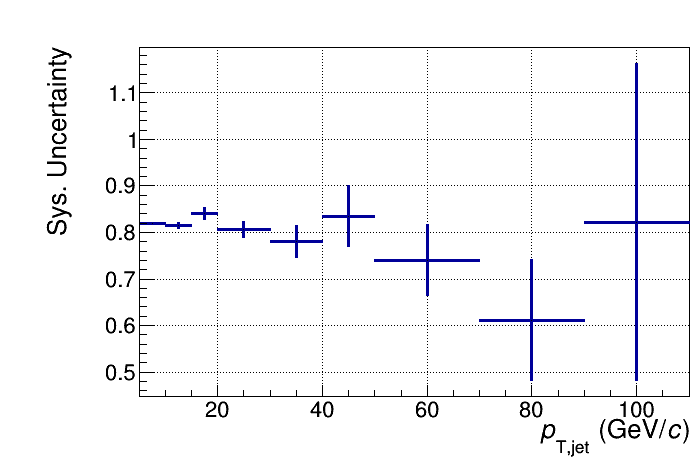
\includegraphics[width=0.5\textwidth]{SysR02_TrkEff} &
    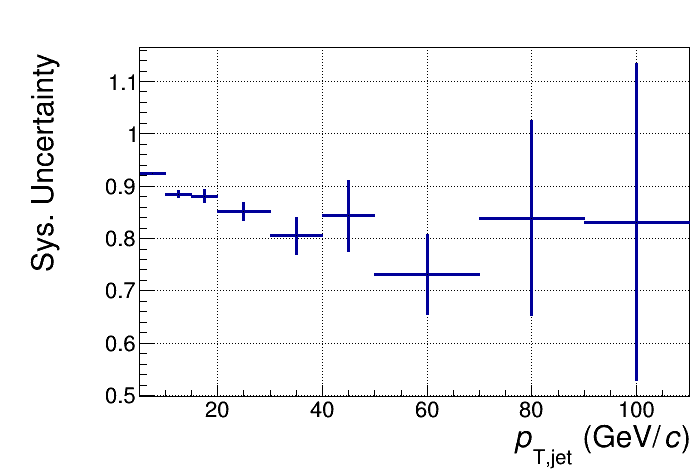
\includegraphics[width=0.5\textwidth]{SysR03_TrkEff}\\
    \multicolumn{2}{c}{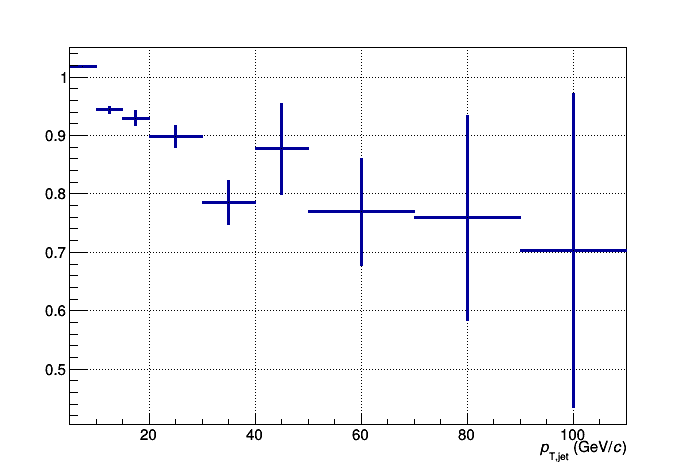
\includegraphics[width=0.5\textwidth]{SysR04_TrkEff}}
\end{array}$
\caption[Systematic due to TPC tracking efficiency.]{\label{fig:trkeff}Systematic due to TPC tracking efficiency.}
\end{figure*}

\noindent
Figure \ref{fig:trkeff} shows the systematical uncertainties for R = 0.2 (top left), R = 0.3 (top right), and R = 0.4 (bottom) jets.   

\subsubsection{Hadronic Correction}

\subsubsection{EMCal Clusterization Algorithm}
\subsection{Systematic Uncertainty to Jet Yield}



\subsubsection{Luminosity Uncertainty}

The luminosity of a hadronic collider, $\mathscr{L}$, is given by the expression



\begin{equation}
\mathscr{L} = \frac{R}{\sigma}
\label{eq:xlumdef}
\end{equation}

\noindent
where R is the interaction rate and $\sigma$ is the visible cross section.  Due to the fact that we only measure events within a 10 cm window within the primary vertex region we must scale the total luminosity to that which is delievered within the primary vertex region of the ALICE experiment.  This scale factor is determined by dividing the total number of MB events to those accepted within the 10 cm window.  $N^{tot}_{MB} / N^{10 cm vertex}_{MB}$ = 1.024 from the acceptance criteria held in this analysis.
The luminosity along with its uncertainty were determined during a a special Van der Meer scan run in April of 2012\cite{ALICE-PUBLIC-2017-002}.  The total systematic uncertainty for the minimum bias (MB) trigger were obtained by measuring the visible cross section using the T0 and V0 detectors.  The MB trigger was defined as V0AND which required a hit in both tjhe V0A and V0C.  The cross section was reported as being a combined average for MB with the V0AND as, 

\begin{equation}
\sigma_{V0} = (55.8 \pm 1.2) mb
\label{eq:xlumdef}
\end{equation}

\noindent
with a combined systematic uncertainty of 2.19\% on the visible cross section and 2.60\% on the luminosity. 


\subsection{Total Uncertainty}

A summary of the total systematic errors used in the final analysis.

\begin{tabular}{ |p{5cm}||p{3cm}|p{3cm}|p{3cm}|  }
 \hline
 \multicolumn{4}{|c|}{Systematic Errors} \\
 \hline
 Systematic &R = 0.2 Jets & R = 0.3 Jets& R = 0.4 Jets\\
 \hline
Sensitivity to Clusterization   & AF    &AFG&   004\\
Hadronic Correction&   AX  & ALA   &248\\
Tracking Efficency &AL & ALB&  008\\
Sensitivity to Unfolding&DZ & DZA&  012\\
Momentum Resolution&   AS  & ASM&016\\
Energy Resolution& AND   &020 & 02\\
 Angola& AO  & AGO&024\\
 \hline

\end{tabular}
\noindent

The systematics from the yield and JES are added in quadrater together and this is combined in quardrater with the statistical errors.

\section{Corrected pp jet cross section}


\subsection{Comparisons to pQCD predictions}

\subsection{Jet Cross Sections and Ratios}



